\documentclass[a4paper]{report}
\usepackage[utf8]{inputenc}
\usepackage[portuguese]{babel}
\usepackage{hyperref}
\usepackage{a4wide}
\hypersetup{pdftitle={LI4 - PL1 - Grupo 1},
pdfauthor={João Teixeira, José Ferreira, Maria Silva, Miguel Solino, Pedro Oliveira},
colorlinks=true,
urlcolor=blue,
linkcolor=black}
\usepackage{subcaption}
\usepackage[cache=false]{minted}
\usepackage{listings}
\usepackage{booktabs}
\usepackage{multirow}
\usepackage{appendix}
\usepackage{tikz}
\usepackage{authblk}
\usepackage{bashful}
\usepackage{verbatim}
\usepackage{amsmath}
\usepackage{amssymb}
\usepackage{multirow}
\usepackage{mwe}
\usetikzlibrary{arrows,%
                petri,%
                topaths}%
\usetikzlibrary{positioning,automata,decorations.markings}
\AfterEndEnvironment{figure}{\noindent\ignorespaces}
\AfterEndEnvironment{table}{\noindent\ignorespaces}

\definecolor{solarized@base03}{HTML}{002B36}
\definecolor{solarized@base02}{HTML}{073642}
\definecolor{solarized@base01}{HTML}{586e75}
\definecolor{solarized@base00}{HTML}{657b83}
\definecolor{solarized@base0}{HTML}{839496}
\definecolor{solarized@base1}{HTML}{93a1a1}
\definecolor{solarized@base2}{HTML}{EEE8D5}
\definecolor{solarized@base3}{HTML}{FDF6E3}
\definecolor{solarized@yellow}{HTML}{B58900}
\definecolor{solarized@orange}{HTML}{CB4B16}
\definecolor{solarized@red}{HTML}{DC322F}
\definecolor{solarized@magenta}{HTML}{D33682}
\definecolor{solarized@violet}{HTML}{6C71C4}
\definecolor{solarized@blue}{HTML}{268BD2}
\definecolor{solarized@cyan}{HTML}{2AA198}
\definecolor{solarized@green}{HTML}{859900}

\lstset{
  language=Java,
  upquote=true,
  columns=fixed,
  tabsize=4,
  extendedchars=true,
  breaklines=true,
  numbers=left,
  numbersep=5pt,
  rulesepcolor=\color{solarized@base03},
  numberstyle=\tiny\color{solarized@base01},
  basicstyle=\footnotesize\ttfamily,
  keywordstyle=\color{solarized@green},
  stringstyle=\color{solarized@yellow}\ttfamily,
  identifierstyle=\color{solarized@blue},
  commentstyle=\color{solarized@base01},
  emphstyle=\color{solarized@red}
}

\begin{document}

\title{Laboratórios de Informática IV\\
\large PL1 - Grupo 1}
\author{José Ferreira (A83683) \and João Teixeira (A85504) \and Maria Silva (A83840) \and Miguel Solino (A86435) \and Pedro Oliveira (A83762)}
\date{\today}

\begin{center}
    \begin{minipage}{0.75\linewidth}
        \centering
        
\includegraphics[width=0.4\textwidth]{images/eng.jpeg}\par\vspace{1cm}
        \vspace{1.5cm}
        \href{https://www.uminho.pt/PT}
        {\color{black}{\scshape\LARGE Universidade do Minho}} \par
        \vspace{1cm}
        \href{https://www.di.uminho.pt/}
        {\color{black}{\scshape\Large Departamento de Informática}} \par
        \vspace{1.5cm}
        \maketitle
    \end{minipage}
\end{center}


\chapter{Resumo}

\tableofcontents

\chapter{Introdução}
    \section{Contextualização}
    \section{Apresentação do Caso de Estudo}
    \section{Motivação e Objetivos}
    \section{Estrutura do Relatório}

\chapter{Fundamentação}
    \section{Definição da Identidade do Sistema}
    \section{Justificação, Viabilidade e Utilidade do Sistema}

\chapter{Planeamento}
    \section{Identificação dos Recursos Necessários}
    \section{Modelação do Sistema a Implementar - Maqueta}
    \section{Definição de Medida de Sucesso}
    \section{Plano de Desenvolvimento}

\chapter{Levantamento de Requisitos}
    \section{Requisitos Funcionais}
    \section{Requisitos Não Funcionais}

\chapter{Modelo de Domínios}

\chapter{Diagrama de Use Cases}
    \begin{figure}[H]
    \centering
        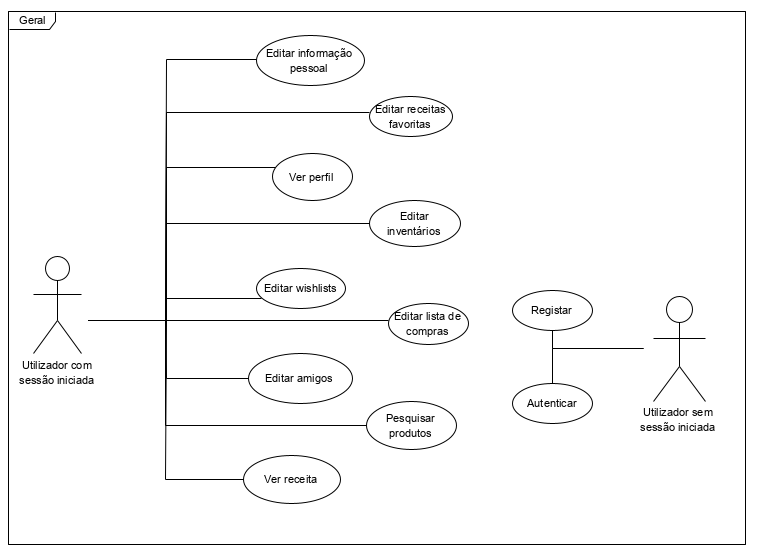
\includegraphics[width=\textwidth]{images/diagrama_use_cases.png}
    \end{figure}

\chapter{Especificação de Use Cases}
    \section{Registar}
        \begin{figure}[H]
        \centering
            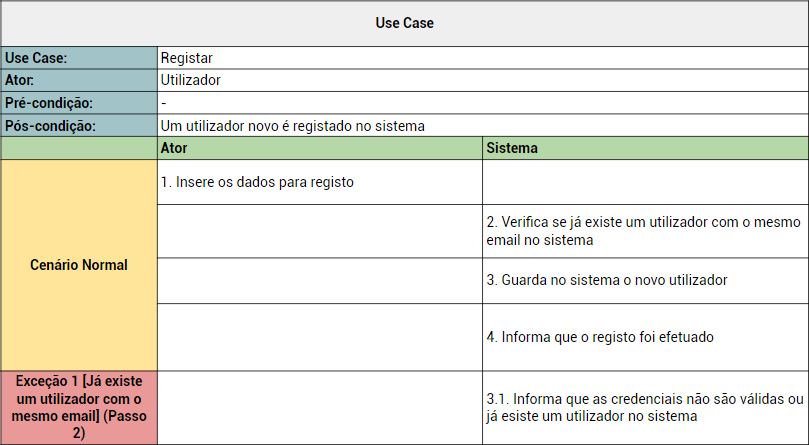
\includegraphics[width=\textwidth]{images/usecases/registar.png}
        \end{figure}

    \section{Autenticar}
        \begin{figure}[H]
        \centering
            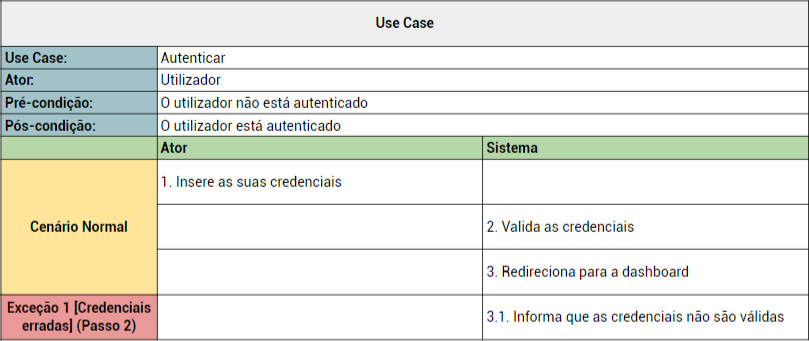
\includegraphics[width=\textwidth]{images/usecases/autenticar.png}
        \end{figure}

    \section{Editar informação pessoal}
        \begin{figure}[H]
        \centering
            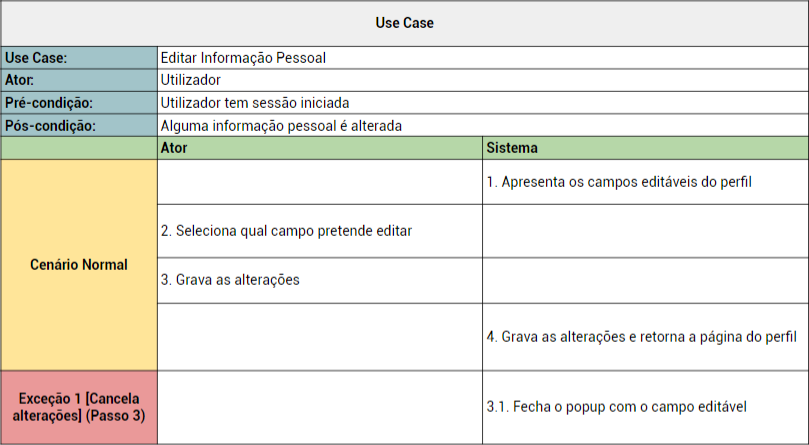
\includegraphics[width=\textwidth]{images/usecases/editar_utilizador.png}
        \end{figure}

    \section{Editar receitas favoritas}
        \begin{figure}[H]
        \centering
            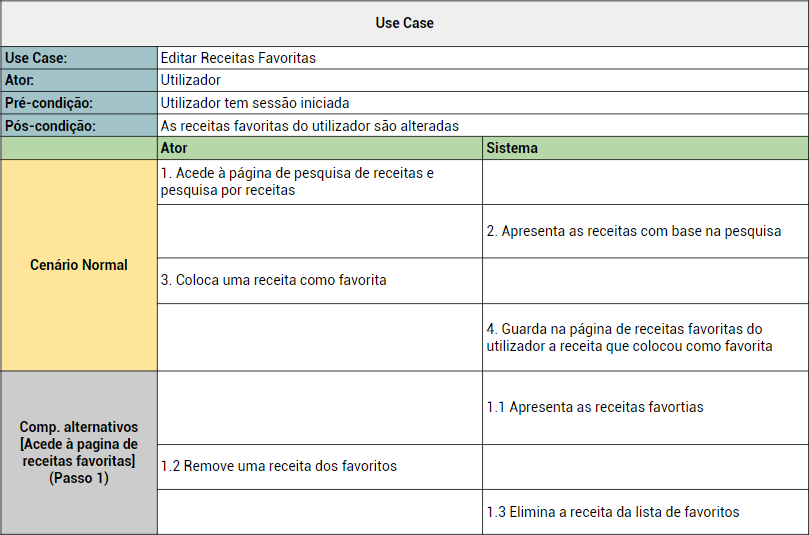
\includegraphics[width=\textwidth]{images/usecases/editar_receitas_favoritas.png}
        \end{figure}

    \section{Ver perfil}
        \begin{figure}[H]
        \centering
            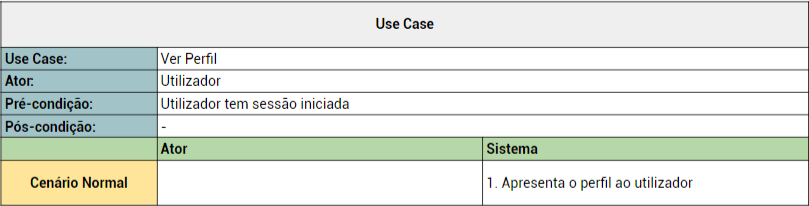
\includegraphics[width=\textwidth]{images/usecases/ver_perfil.png}
        \end{figure}

    \section{Editar inventários}
        \begin{figure}[H]
        \centering
            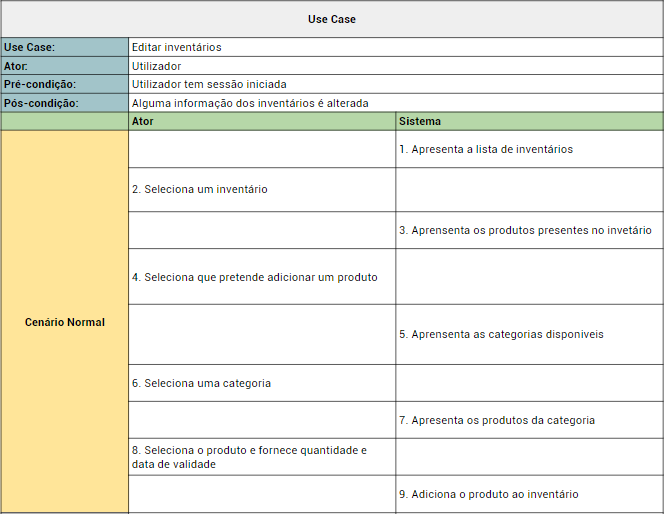
\includegraphics[width=\textwidth]{images/usecases/editar_iventarios_1.png}
            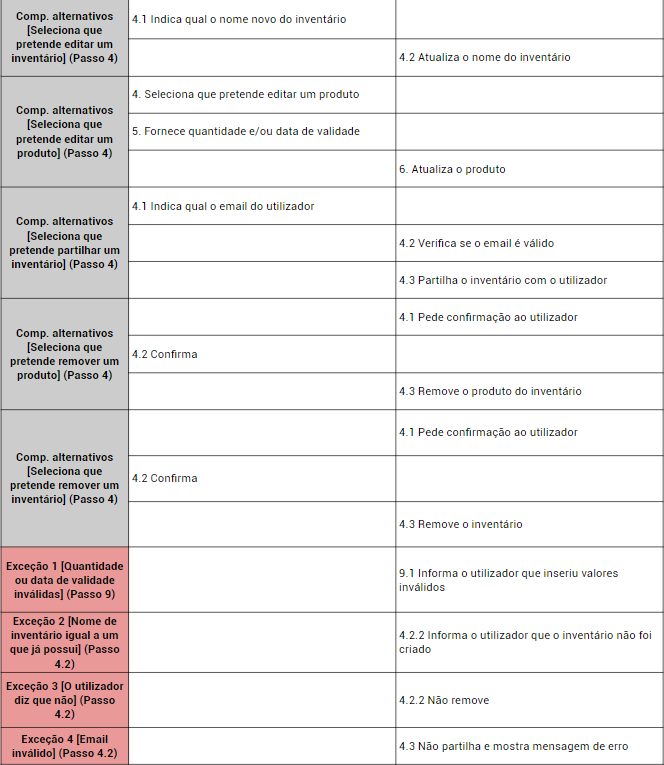
\includegraphics[width=\textwidth]{images/usecases/editar_iventarios_2.png}
        \end{figure}

    \section{Editar wishlists}
        \begin{figure}[H]
        \centering
            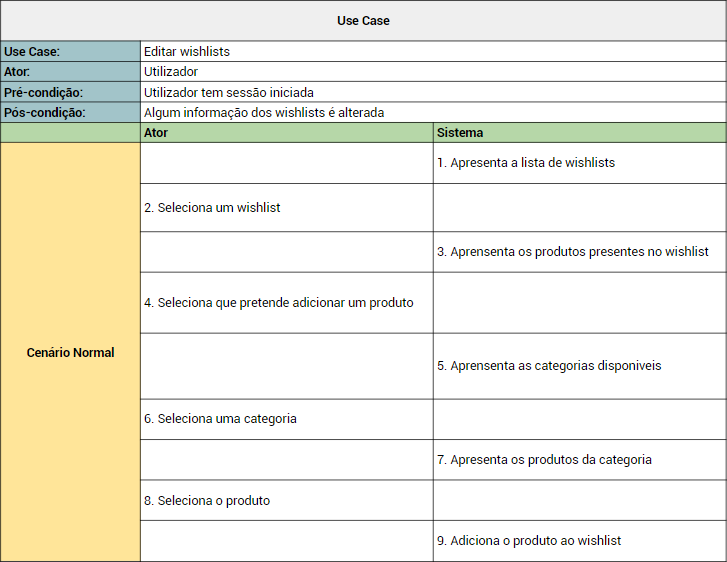
\includegraphics[width=\textwidth]{images/usecases/editar_whishlist_1.png}
            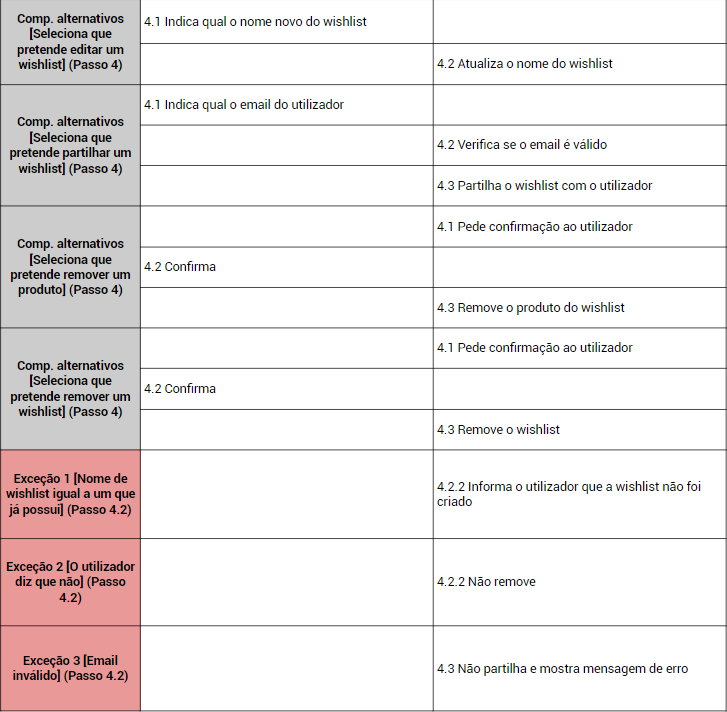
\includegraphics[width=\textwidth]{images/usecases/editar_whishlist_2.png}
        \end{figure}

    \section{Editar listas de compras}
        \begin{figure}[H]
        \centering
            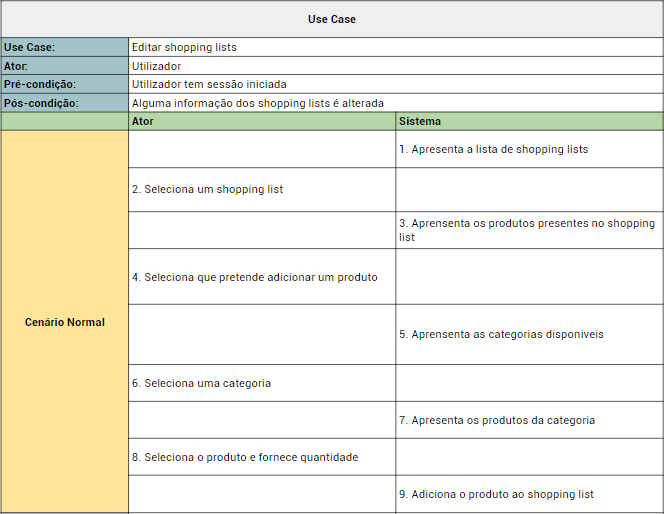
\includegraphics[width=\textwidth]{images/usecases/editar_shoppinglist_1.png}
            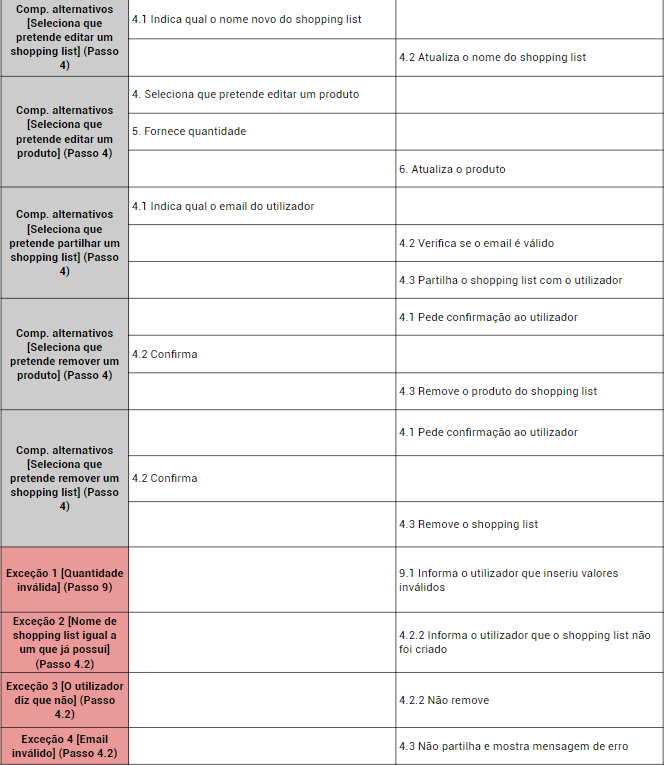
\includegraphics[width=\textwidth]{images/usecases/editar_shoppinglist_2.png}
        \end{figure}

    \section{Editar amigos}
        \begin{figure}[H]
        \centering
            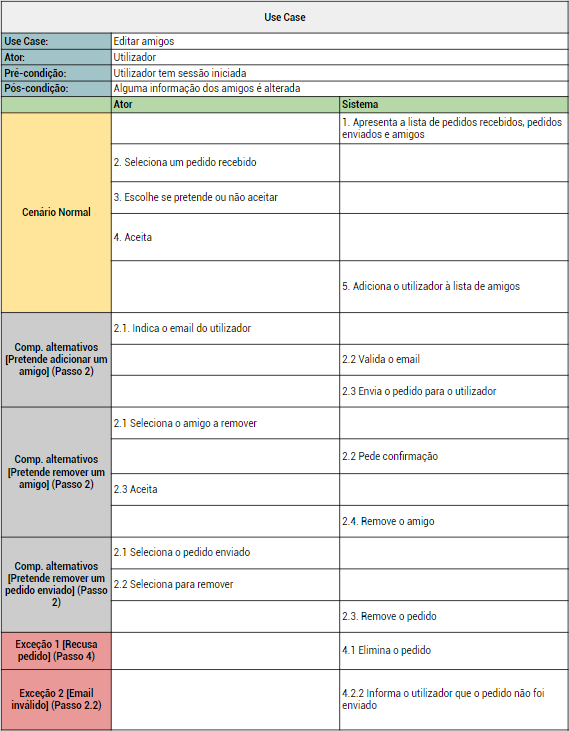
\includegraphics[width=\textwidth]{images/usecases/editar_amigos.png}
        \end{figure}

    \section{Pesquisar produtos}
        \begin{figure}[H]
        \centering
            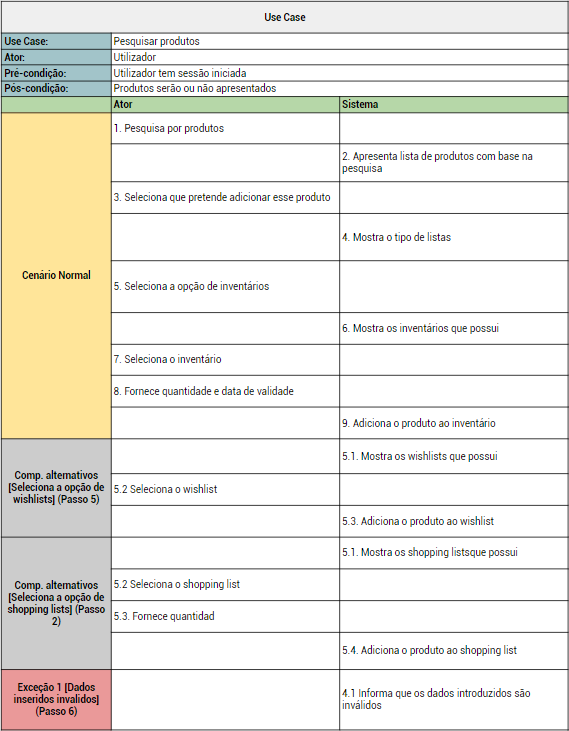
\includegraphics[width=\textwidth]{images/usecases/pesquisar_produto.png}
        \end{figure}

    \section{Ver receita}
        \begin{figure}[H]
        \centering
            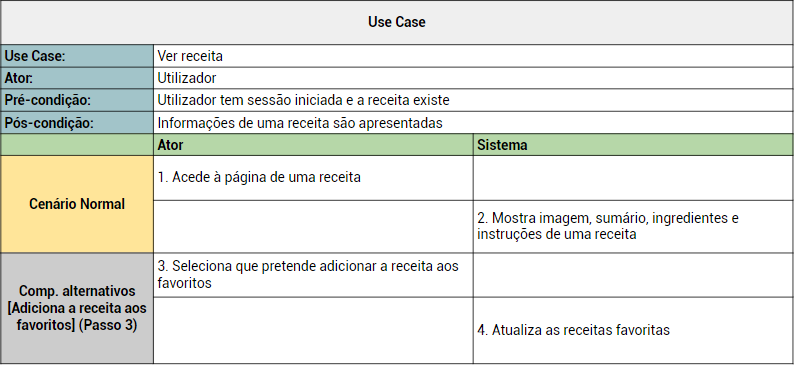
\includegraphics[width=\textwidth]{images/usecases/ver_receita.png}
        \end{figure}

\chapter{Máquina de Estado - Preparar Receita}

\chapter{Arquitetura da Camada de Negócios}
    \section{Camada de Negócios}
    \section{Dicionário das Principais Classes}
    \section{Descrição da Arquitetura}
    \section{Diagrama de Classes}
        \begin{figure}[H]
        \centering
                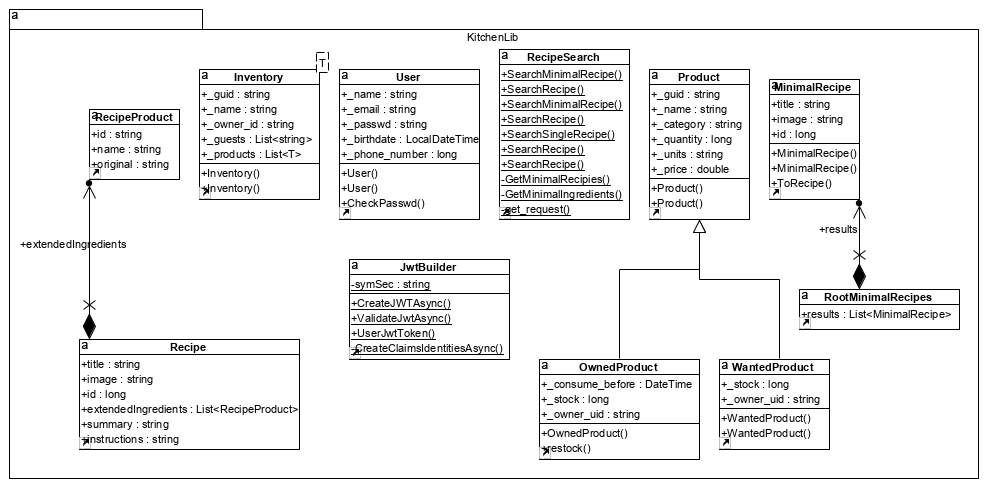
\includegraphics[width=\textwidth]{images/diagrama_de_classes.png}
        \end{figure}

    \section{Diagrama de ORM}
        \begin{figure}[H]
        \centering
            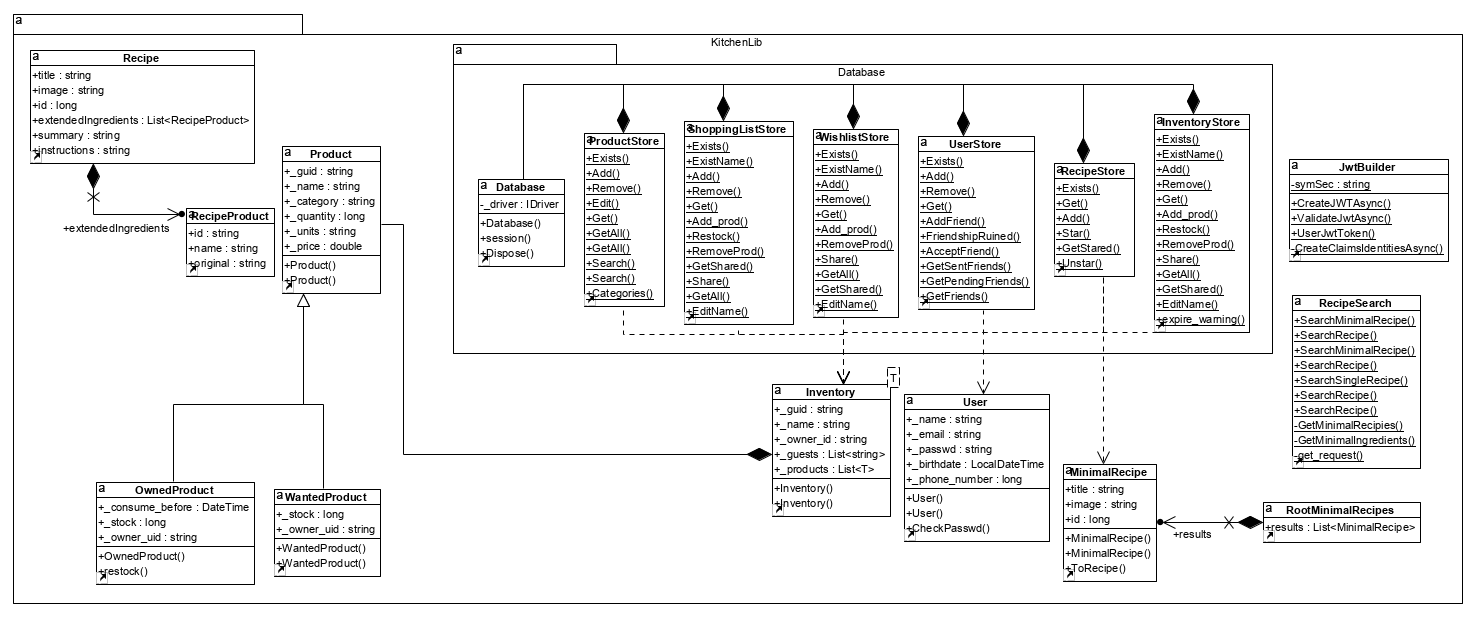
\includegraphics[width=\textwidth]{images/diagrama_de_ORN.png}
        \end{figure}

\chapter{Camada de Dados}
    \section{Modelo Lógico}
    \section{Diagrama de Modelo Lógico}

\chapter{Proposta de Interface}
    \begin{figure}[H]
    \centering
            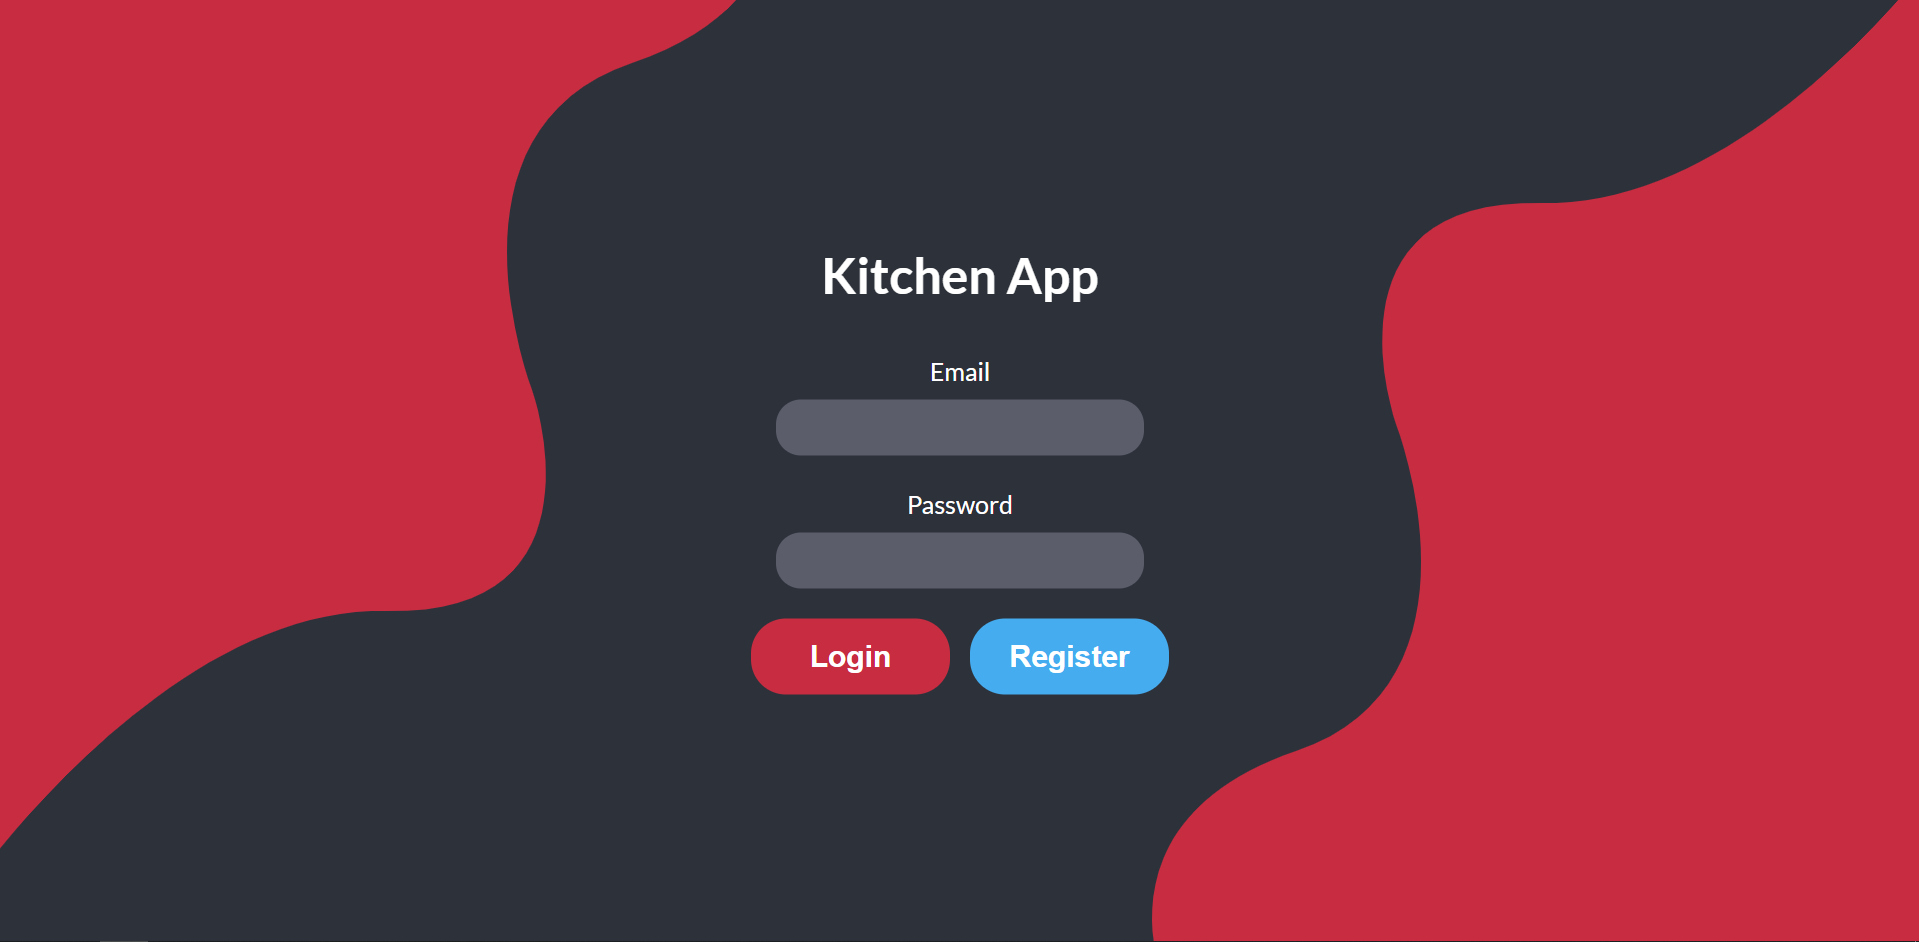
\includegraphics[width=0.7\textwidth]{images/mockup/login_desktop.png}
            \caption{Login no Desktop}
    \end{figure}
    \begin{figure}[H]
    \centering
            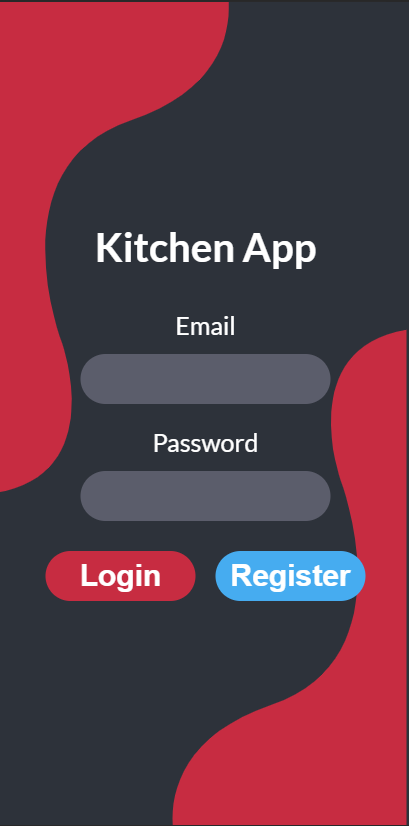
\includegraphics[width=0.2\textwidth]{images/mockup/login_mobile.png}
            \caption{Login em Mobile}
    \end{figure}
    \begin{figure}[H]
    \centering
            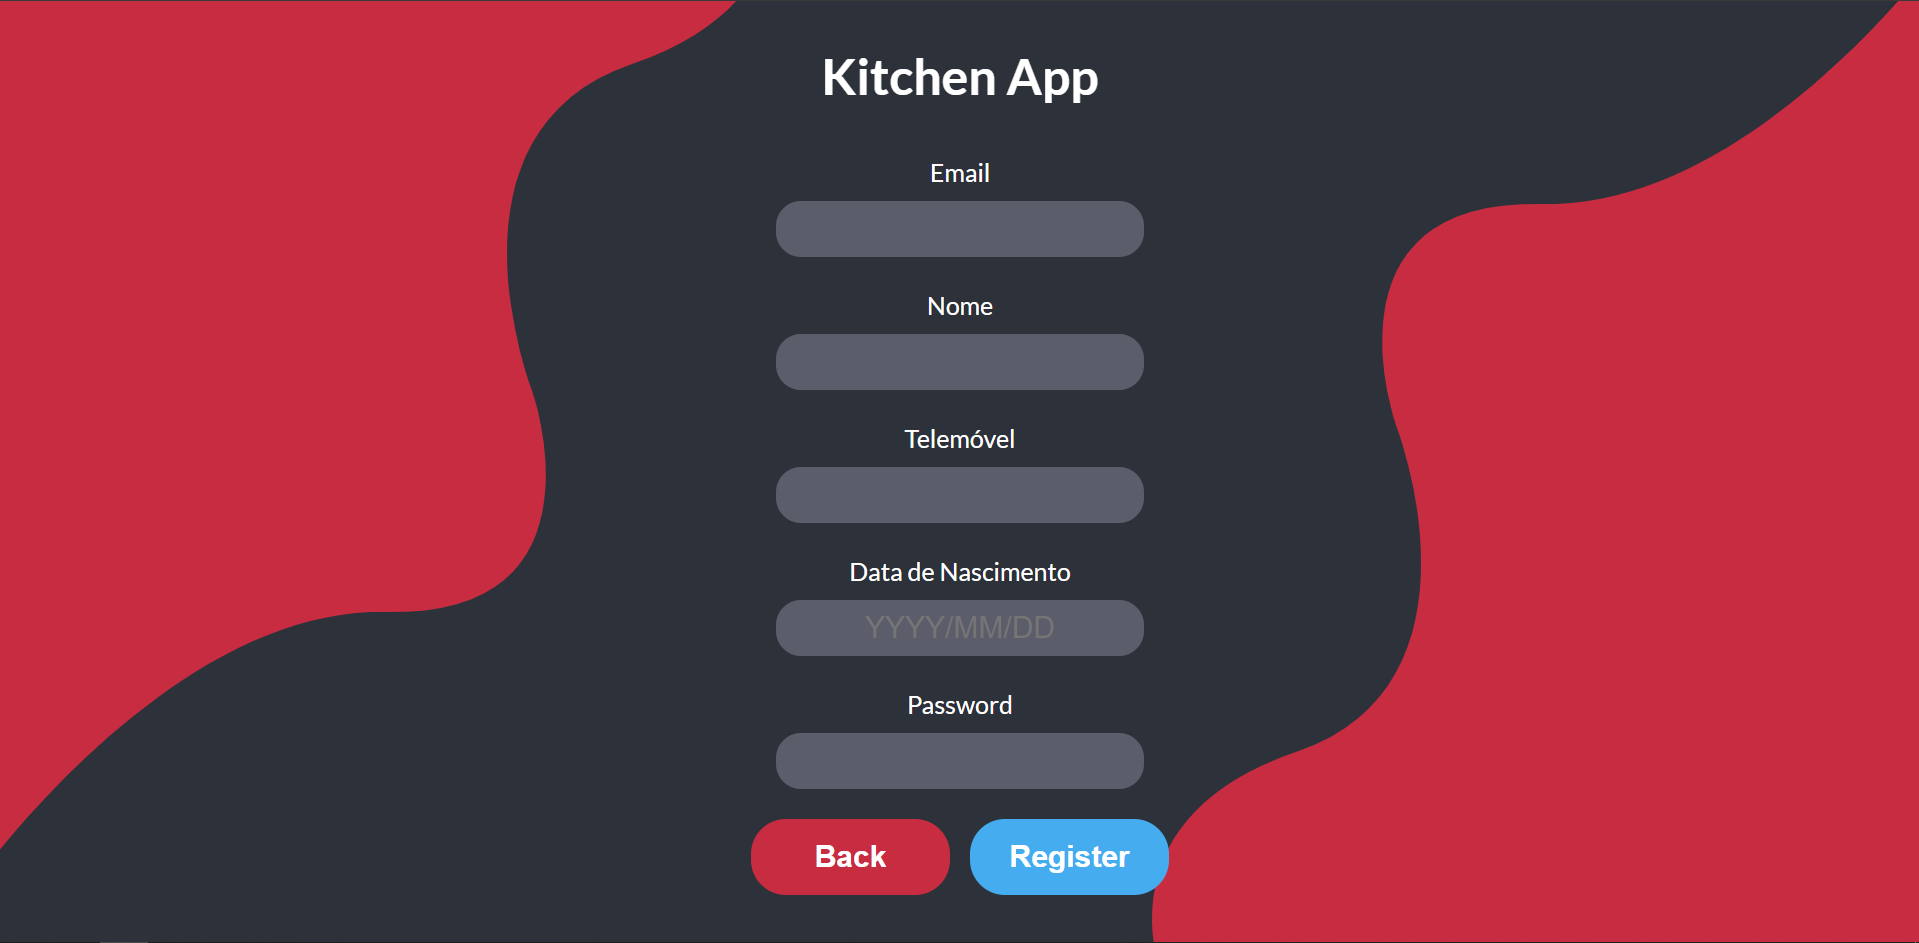
\includegraphics[width=0.7\textwidth]{images/mockup/register_desktop.png}
            \caption{Registo no Desktop}
    \end{figure}
    \begin{figure}[H]
    \centering
            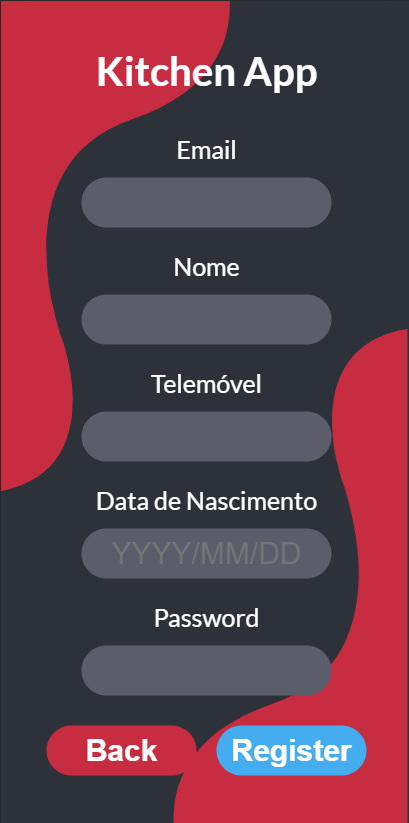
\includegraphics[width=0.2\textwidth]{images/mockup/register_mobile.png}
            \caption{Registo em Mobile}
    \end{figure}
    \begin{figure}[H]
    \centering
            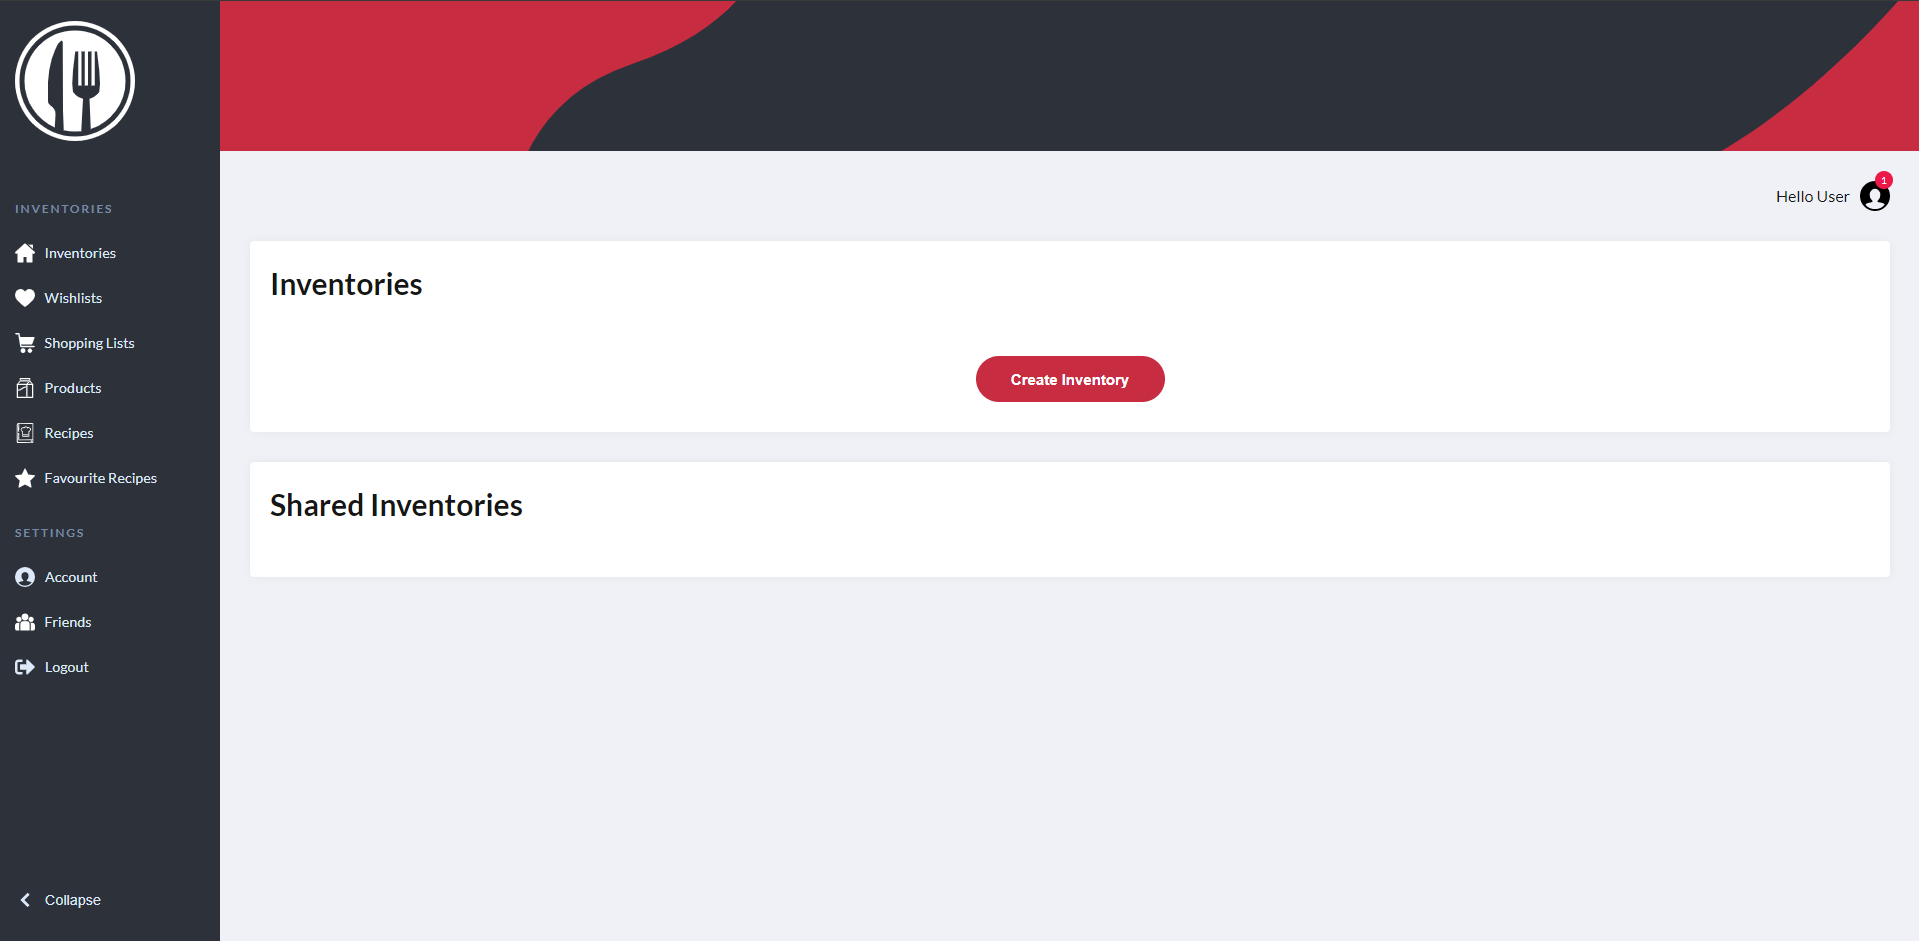
\includegraphics[width=0.7\textwidth]{images/mockup/dashboard_desktop.png}
            \caption{Dashboard no Desktop}
    \end{figure}
    \begin{figure}[H]
    \centering
            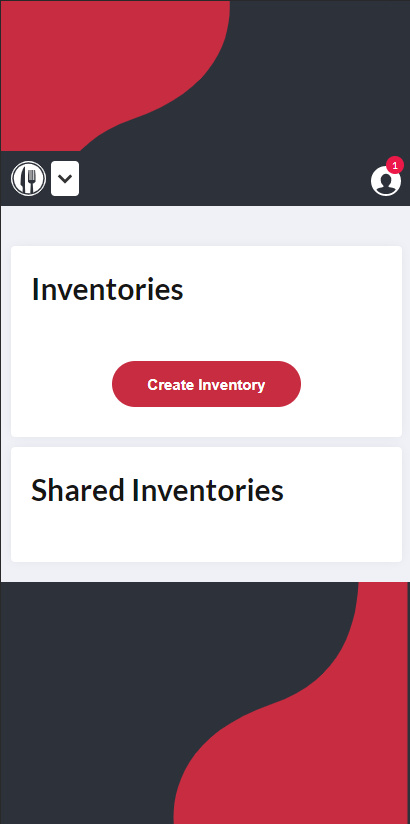
\includegraphics[width=0.2\textwidth]{images/mockup/dashboard_mobile.png}
            \caption{Dashboard em Mobile}
    \end{figure}
    

\chapter{Metodologia de Implementação}

\chapter{Desenvolvimento do Projeto}
    \section{Conexão da Base de Dados}
    \section{API de Receitas}
    \section{Calendarização}

\chapter{Produto Final}
    \begin{figure}[H]
        \centering
            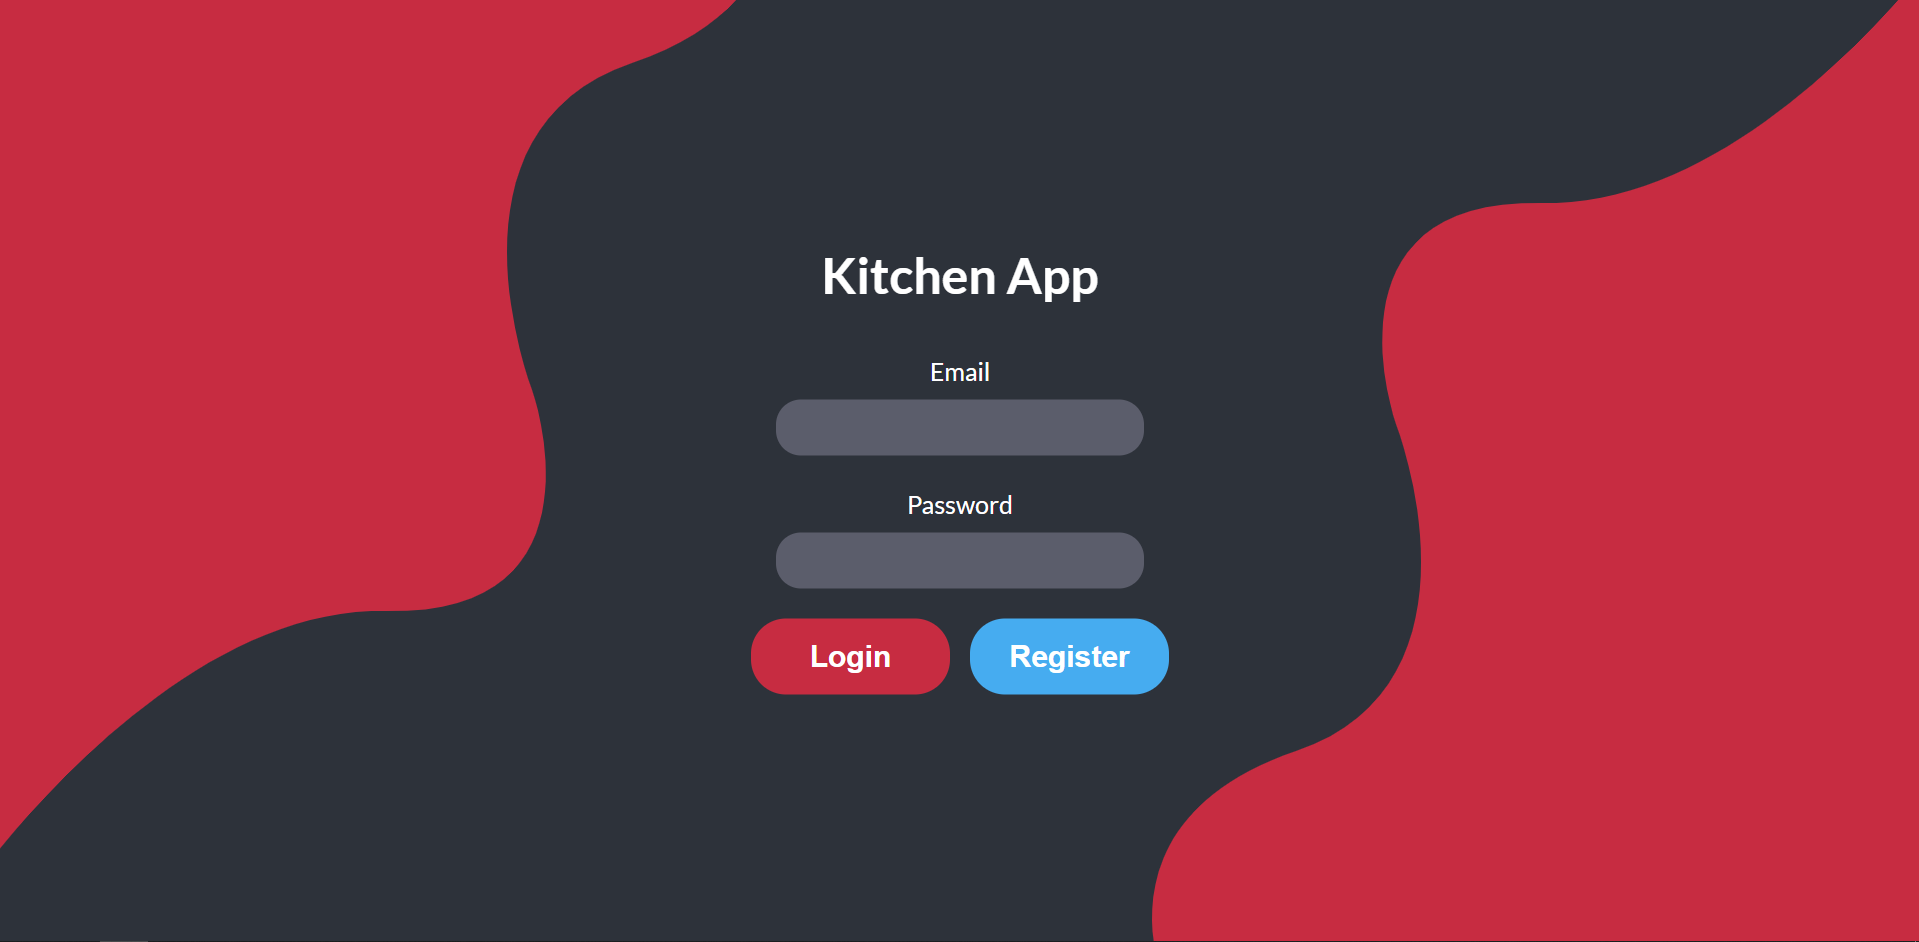
\includegraphics[width=\textwidth]{images/produto_final/login.png}
    \end{figure}

    \begin{figure}[H]
        \centering
            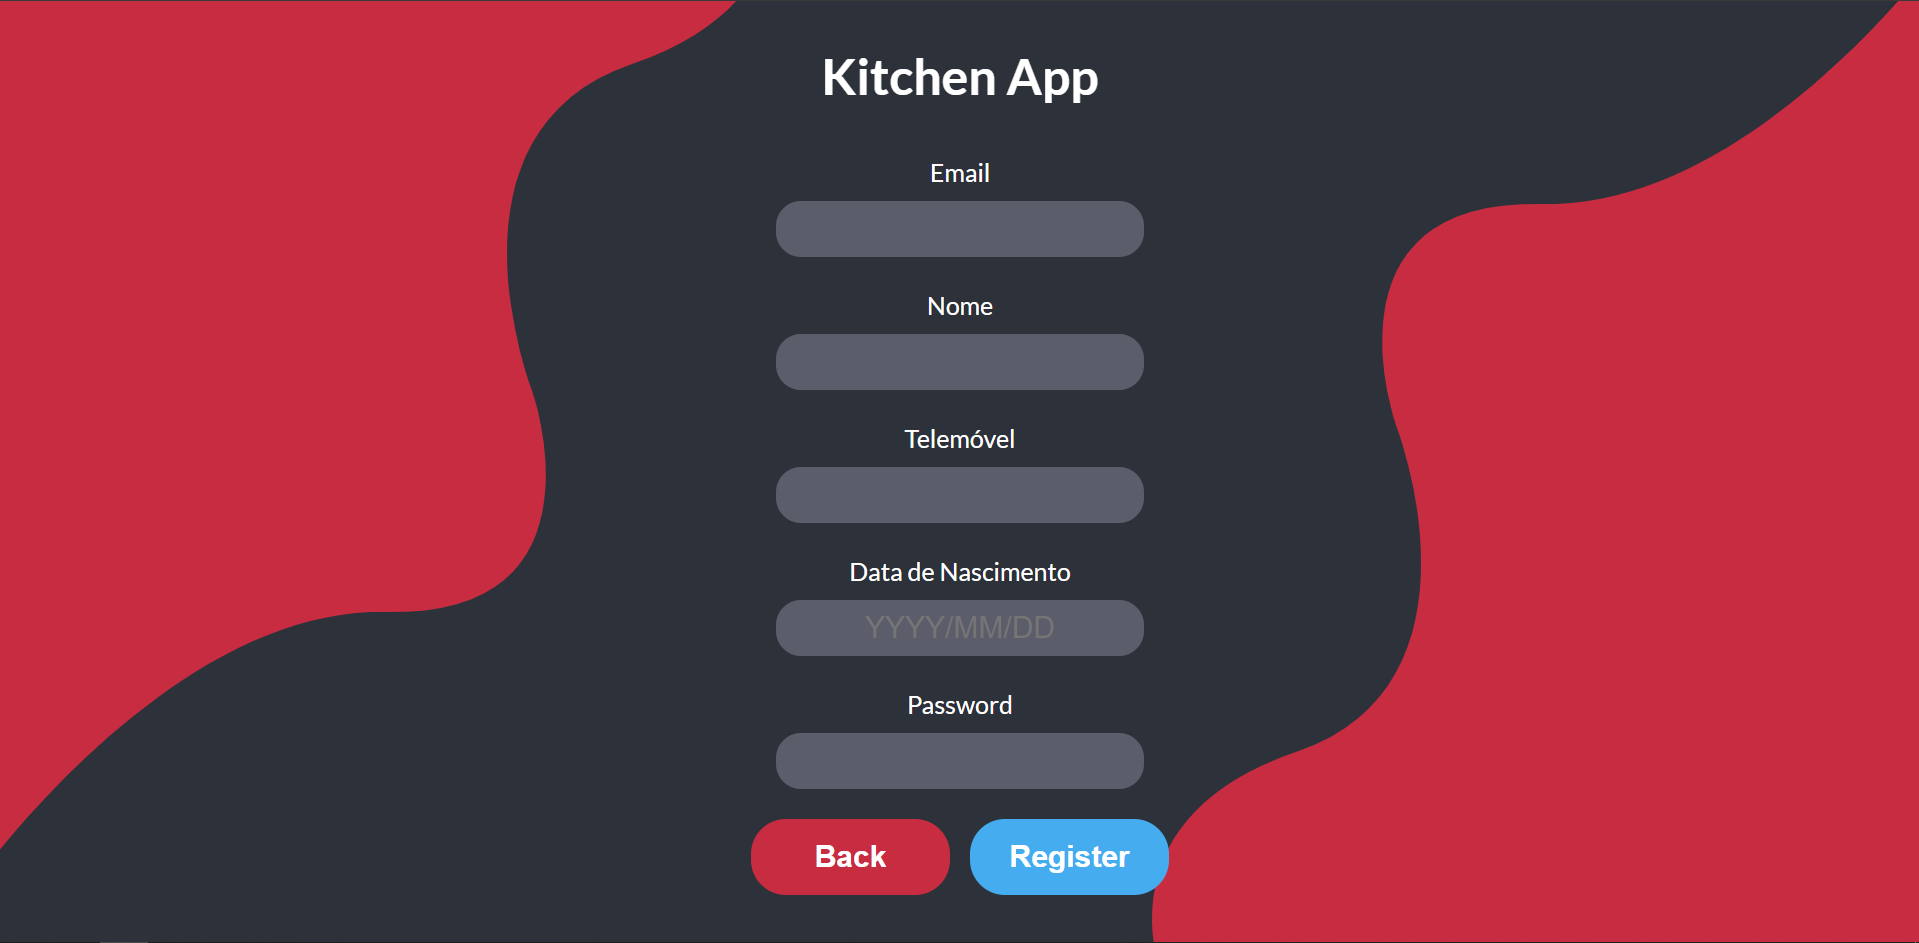
\includegraphics[width=\textwidth]{images/produto_final/registo.png}
    \end{figure}

    \begin{figure}[H]
        \centering
            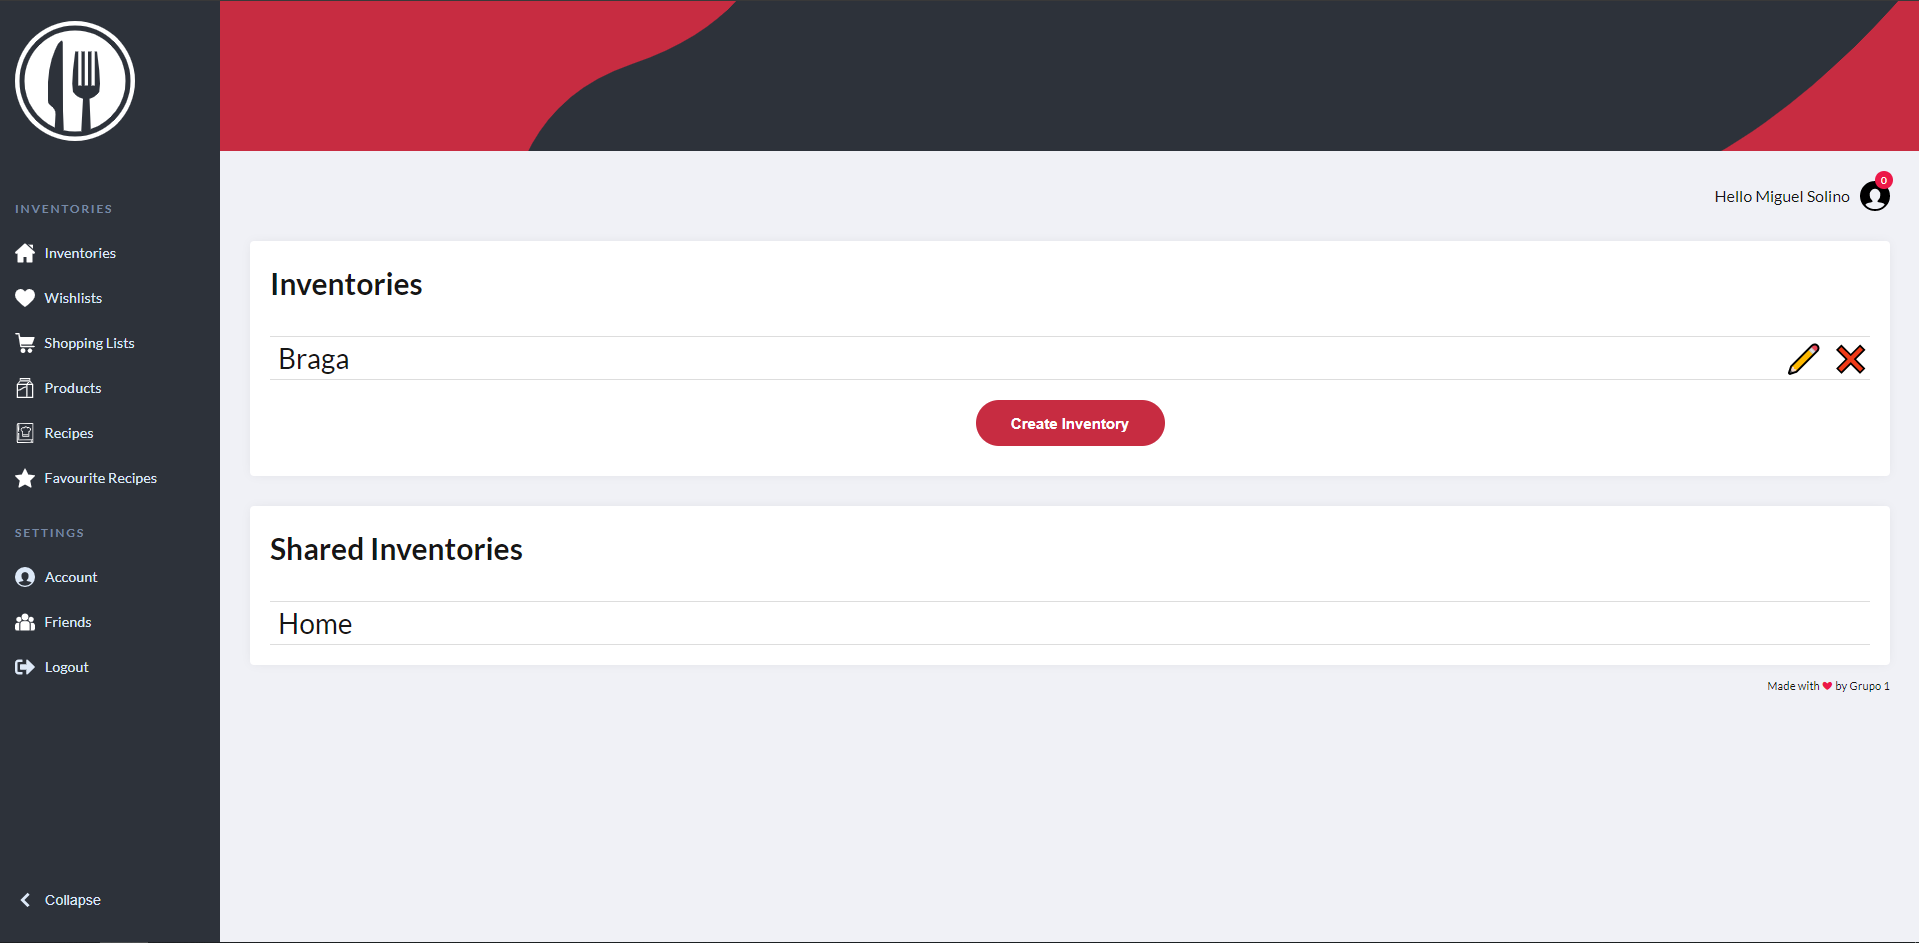
\includegraphics[width=\textwidth]{images/produto_final/inicial.png}
    \end{figure}

    \begin{figure}[H]
        \centering
            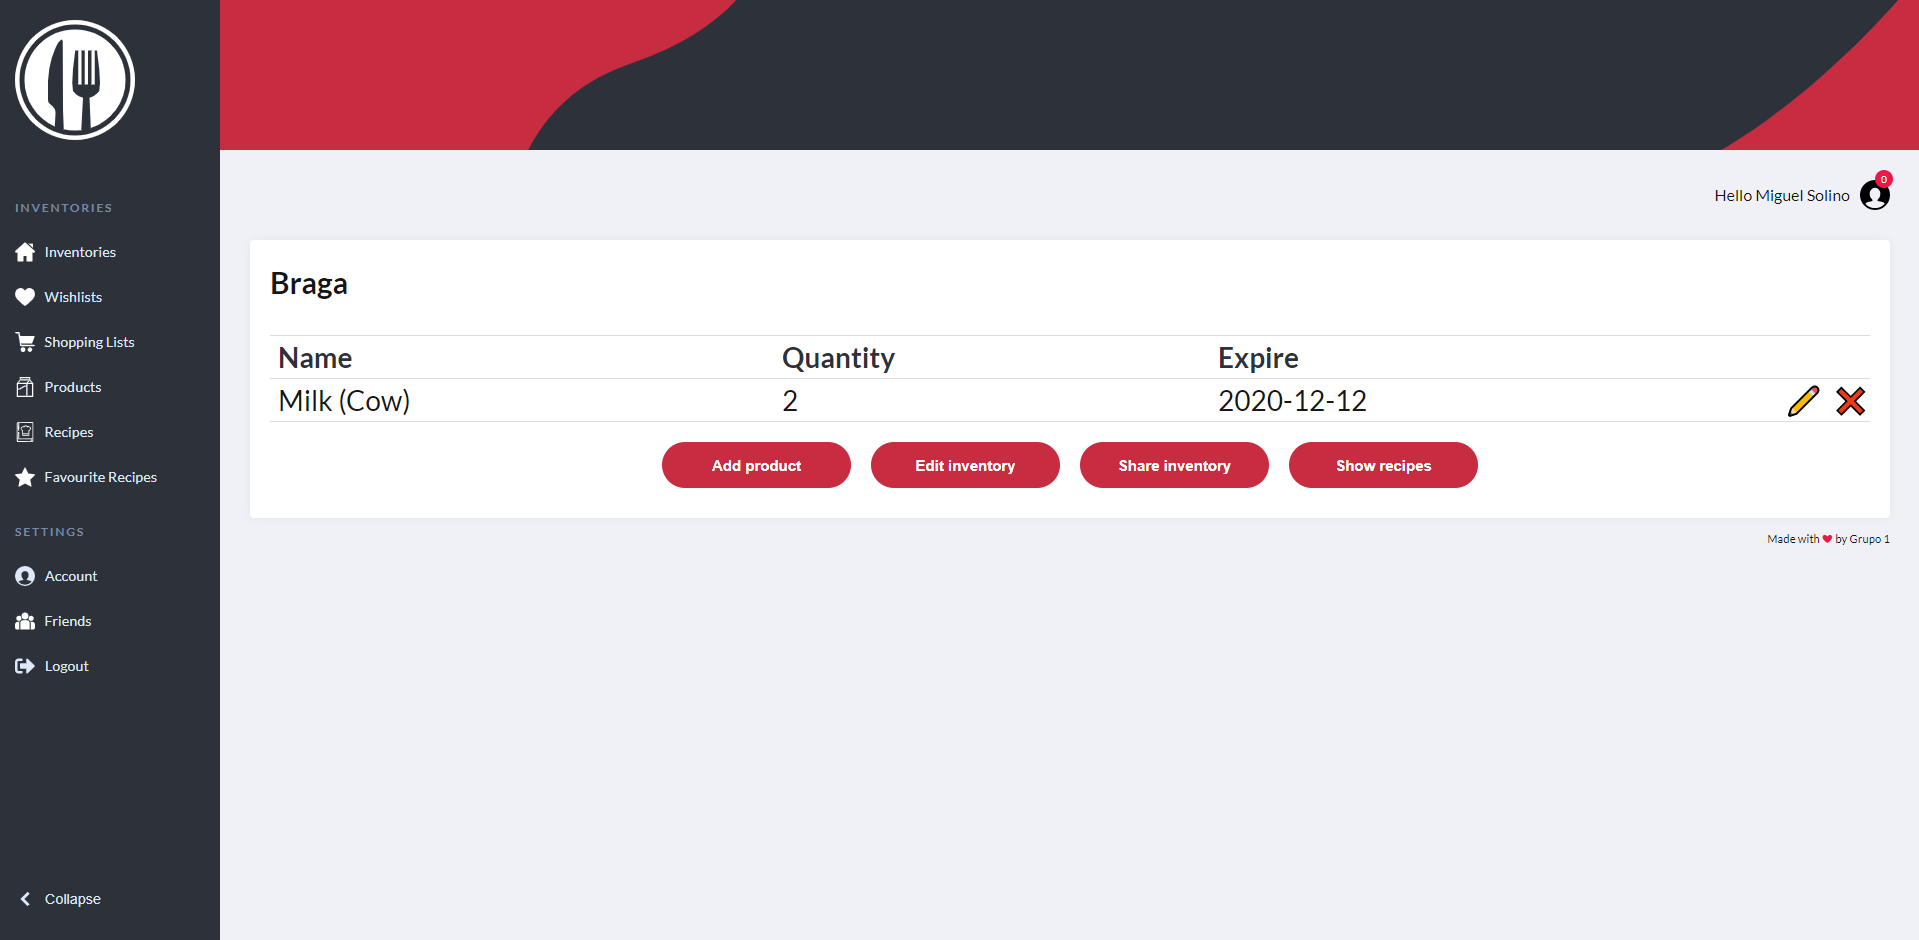
\includegraphics[width=\textwidth]{images/produto_final/iventario.png}
    \end{figure}

    \begin{figure}[H]
        \centering
            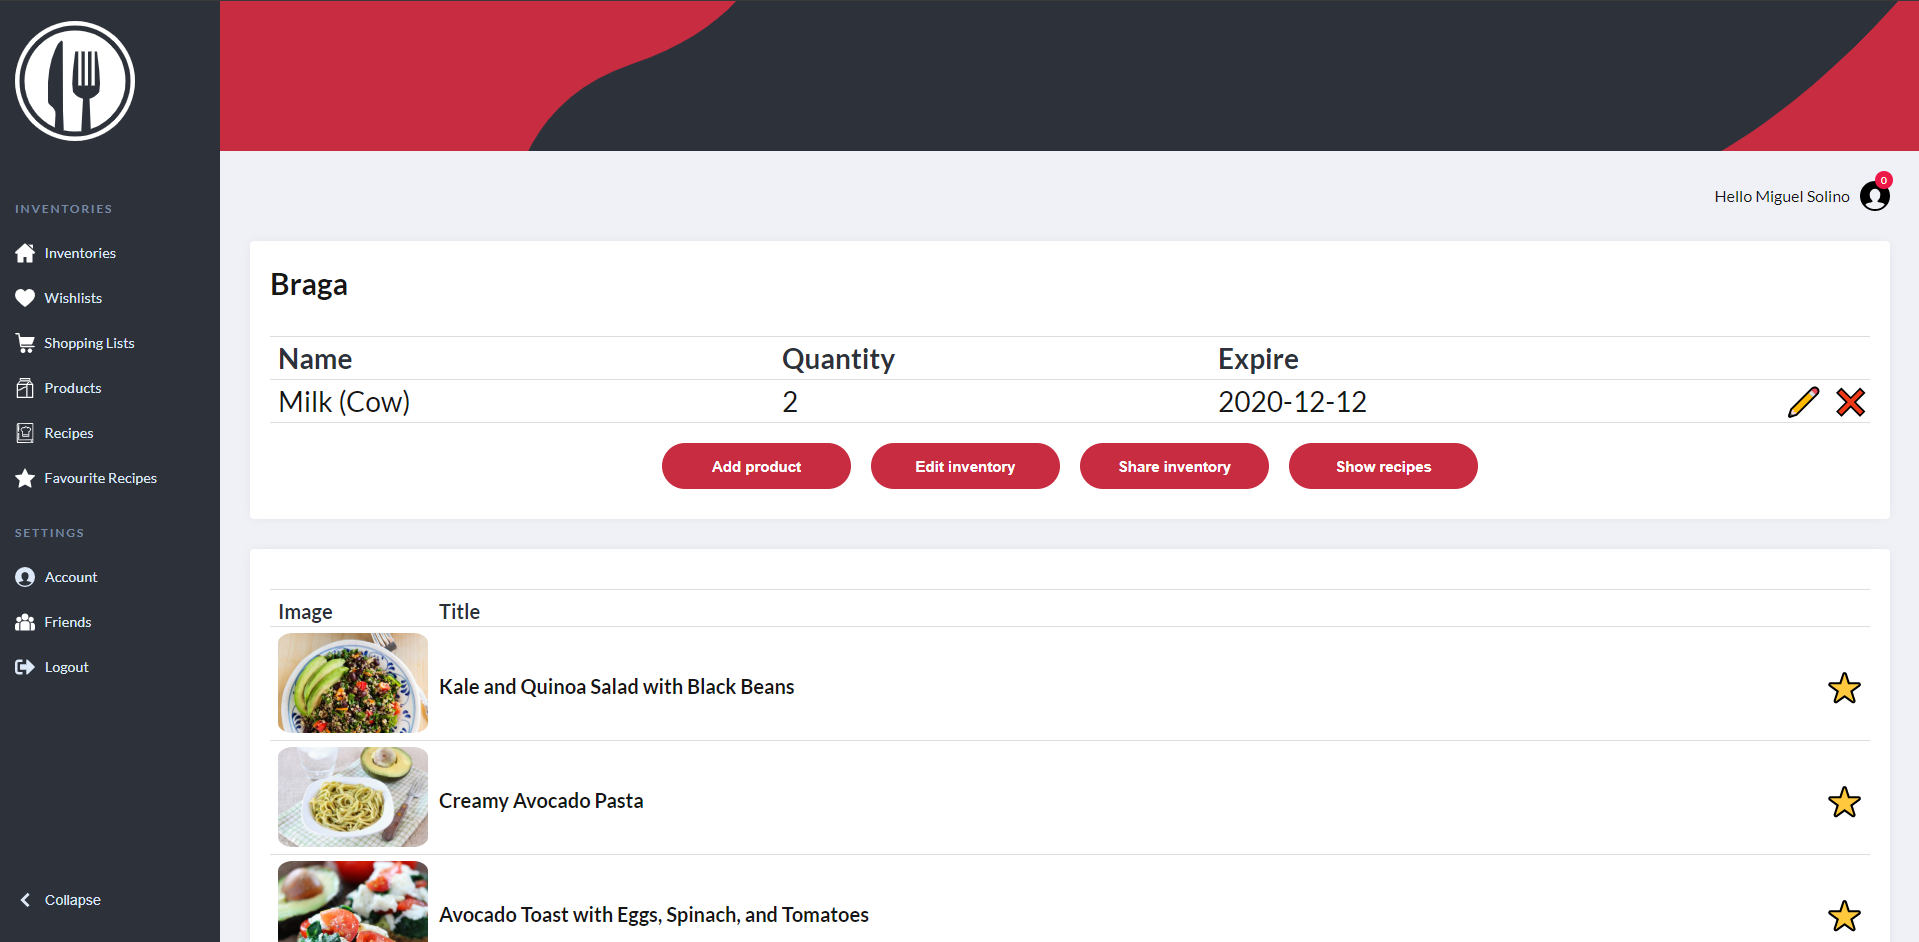
\includegraphics[width=\textwidth]{images/produto_final/iventario_receitas.png}
    \end{figure}

    \begin{figure}[H]
        \centering
            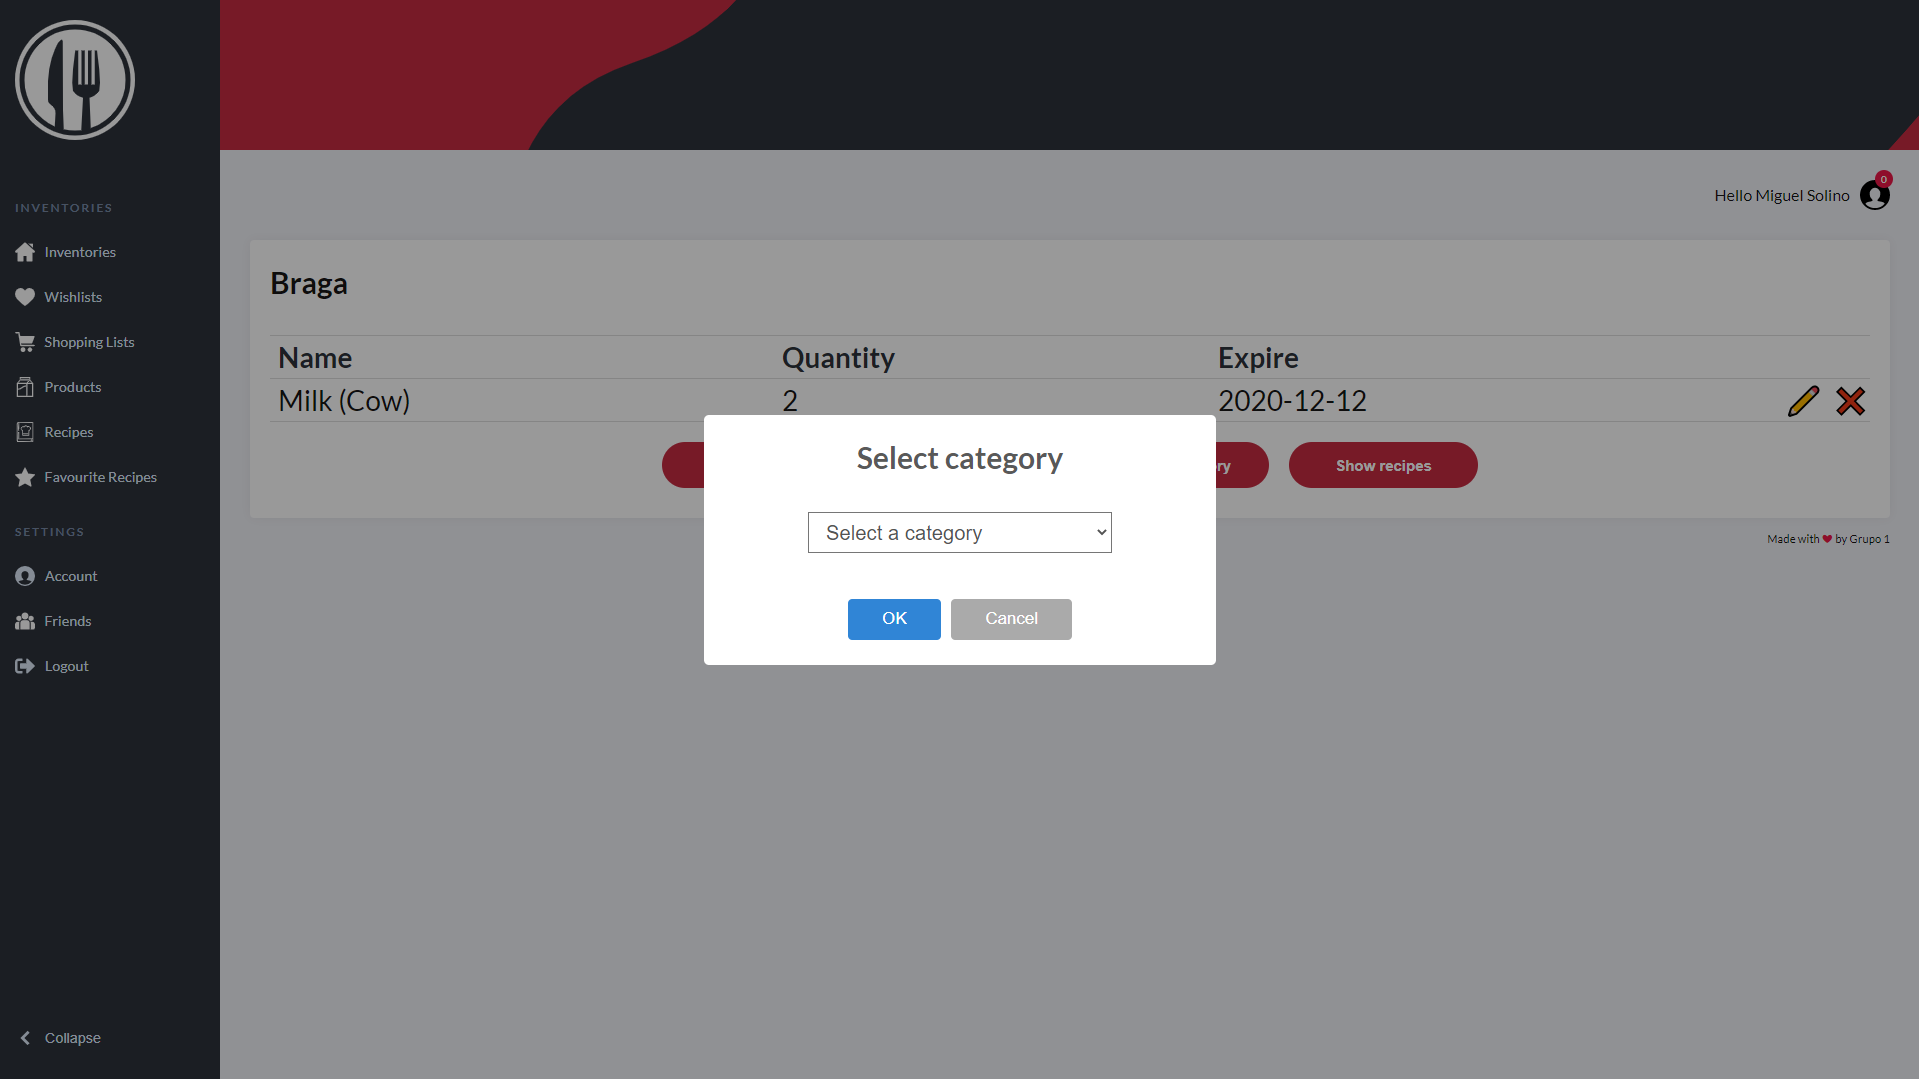
\includegraphics[width=\textwidth]{images/produto_final/inserir_produto_categoria.png}
    \end{figure}

    \begin{figure}[H]
        \centering
            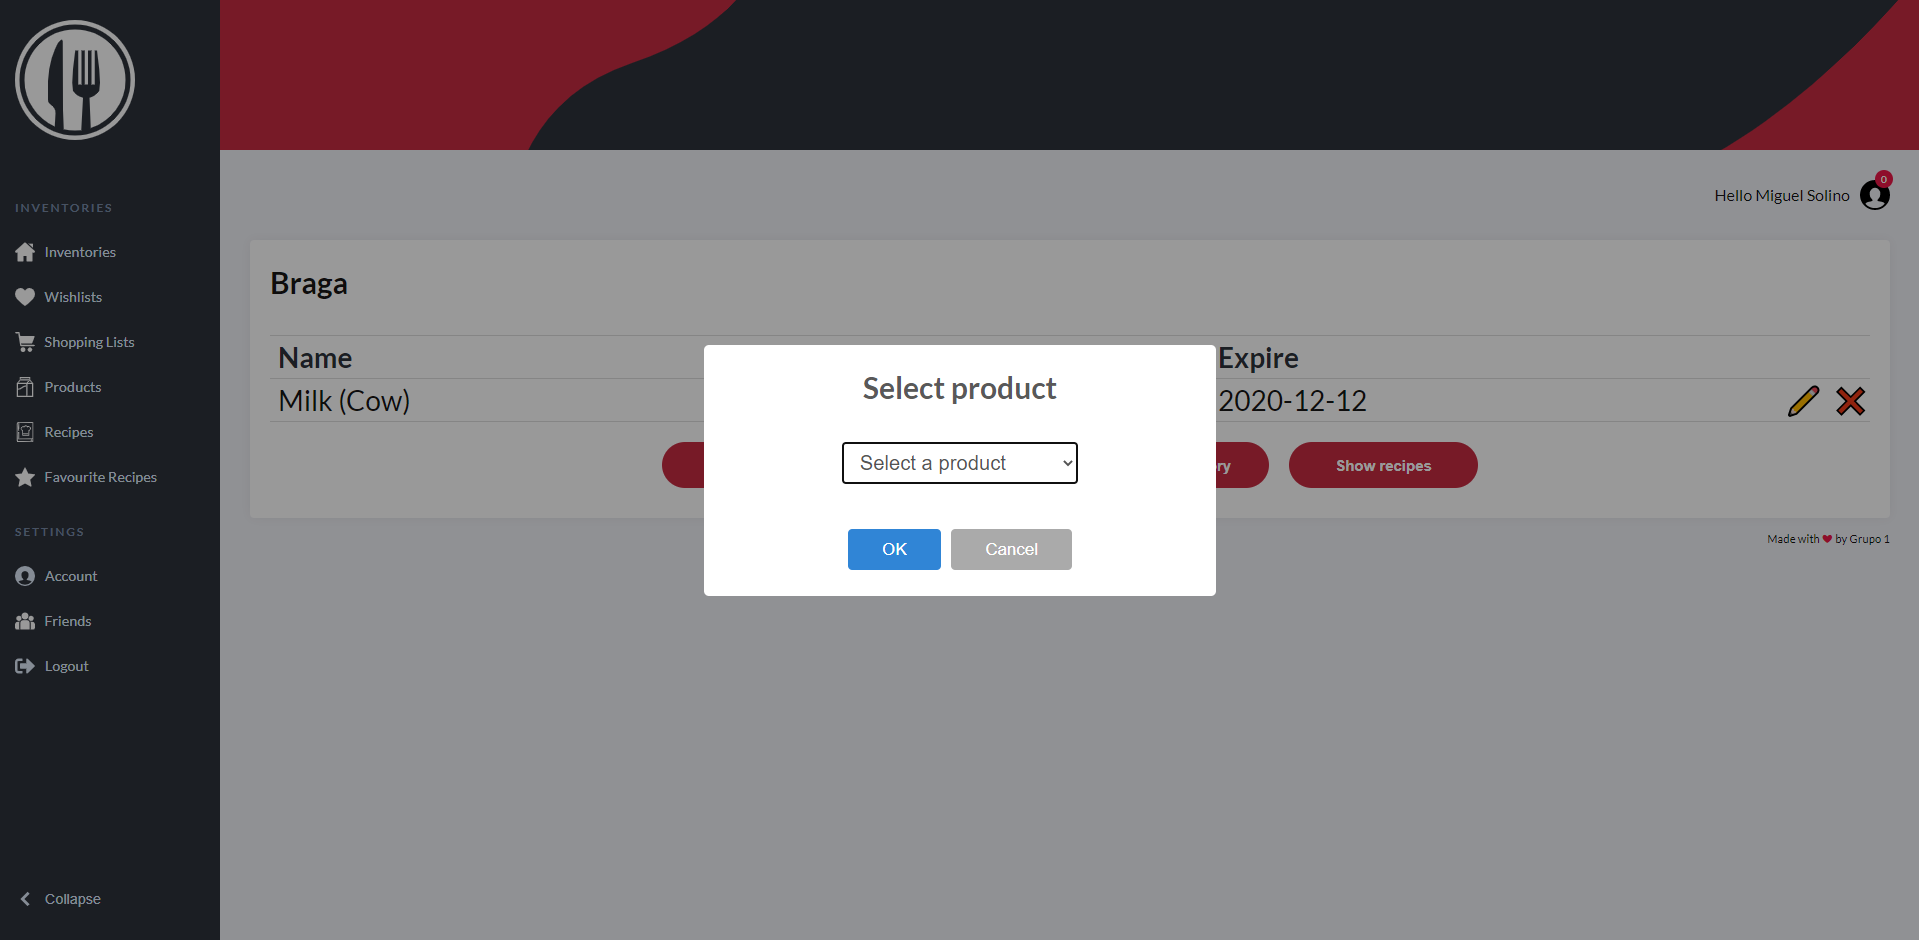
\includegraphics[width=\textwidth]{images/produto_final/inserir_produto_produto.png}
    \end{figure}

    \begin{figure}[H]
        \centering
            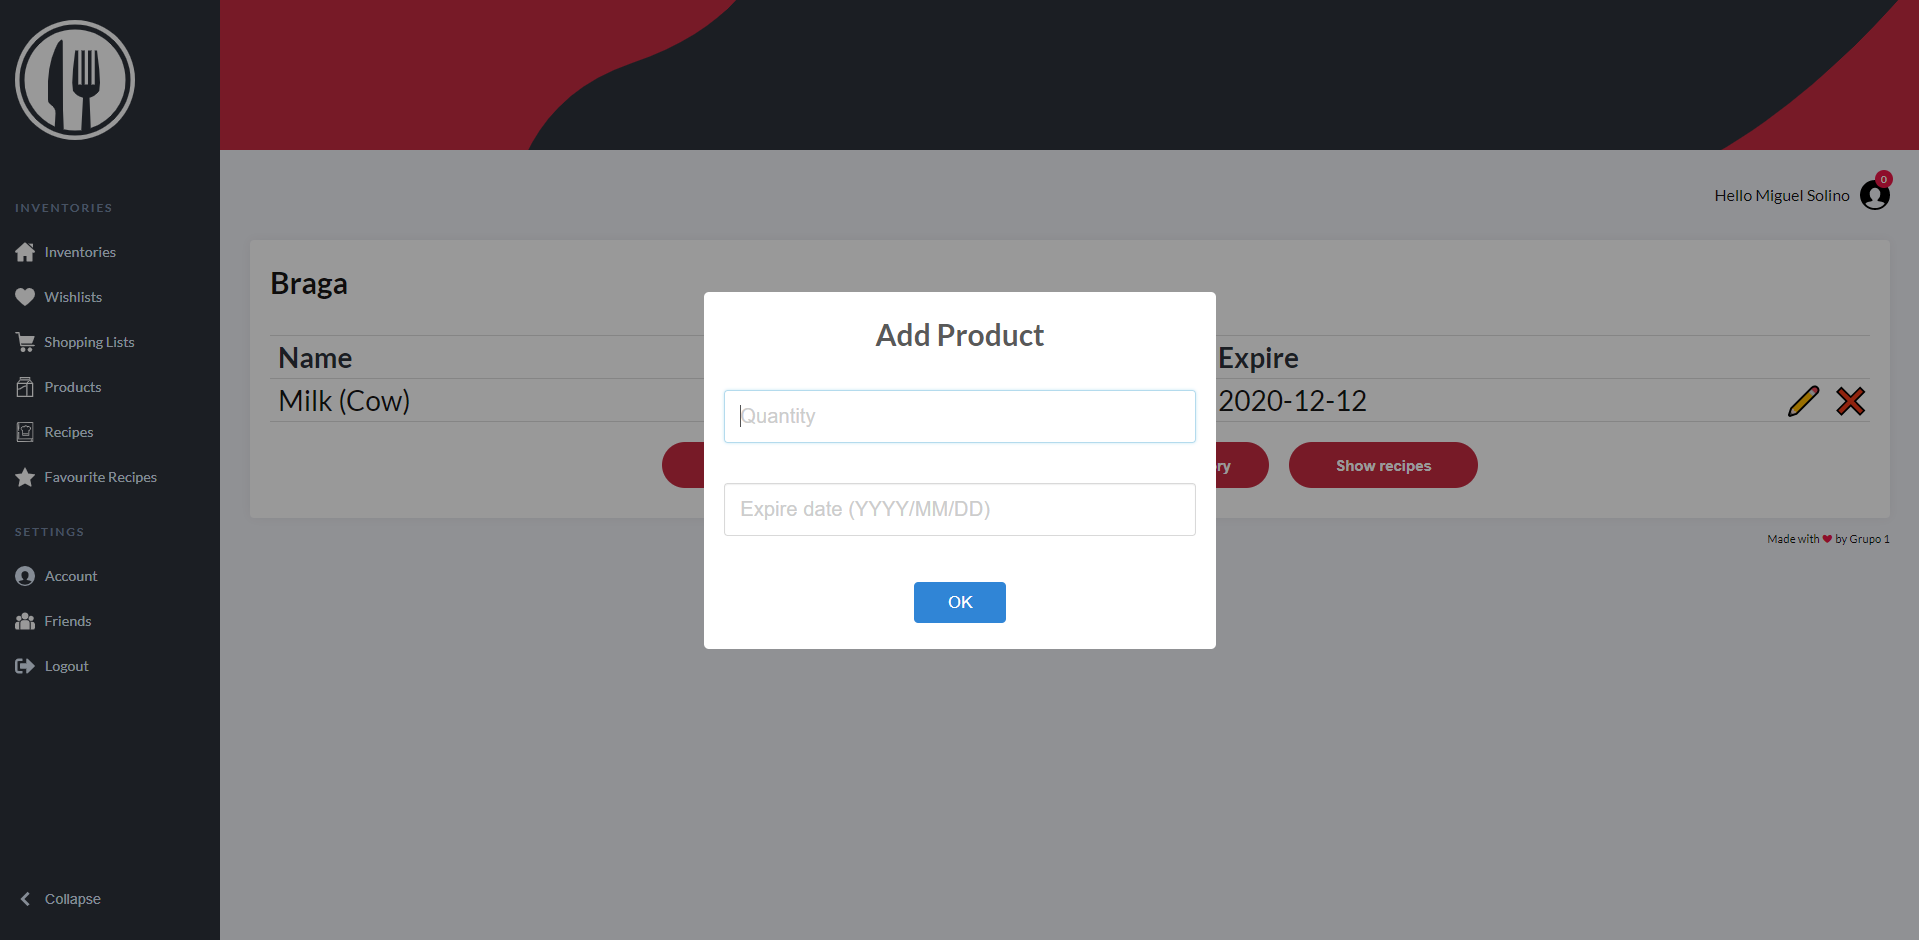
\includegraphics[width=\textwidth]{images/produto_final/inserir_produto_quantidade.png}
    \end{figure}

    \begin{figure}[H]
        \centering
            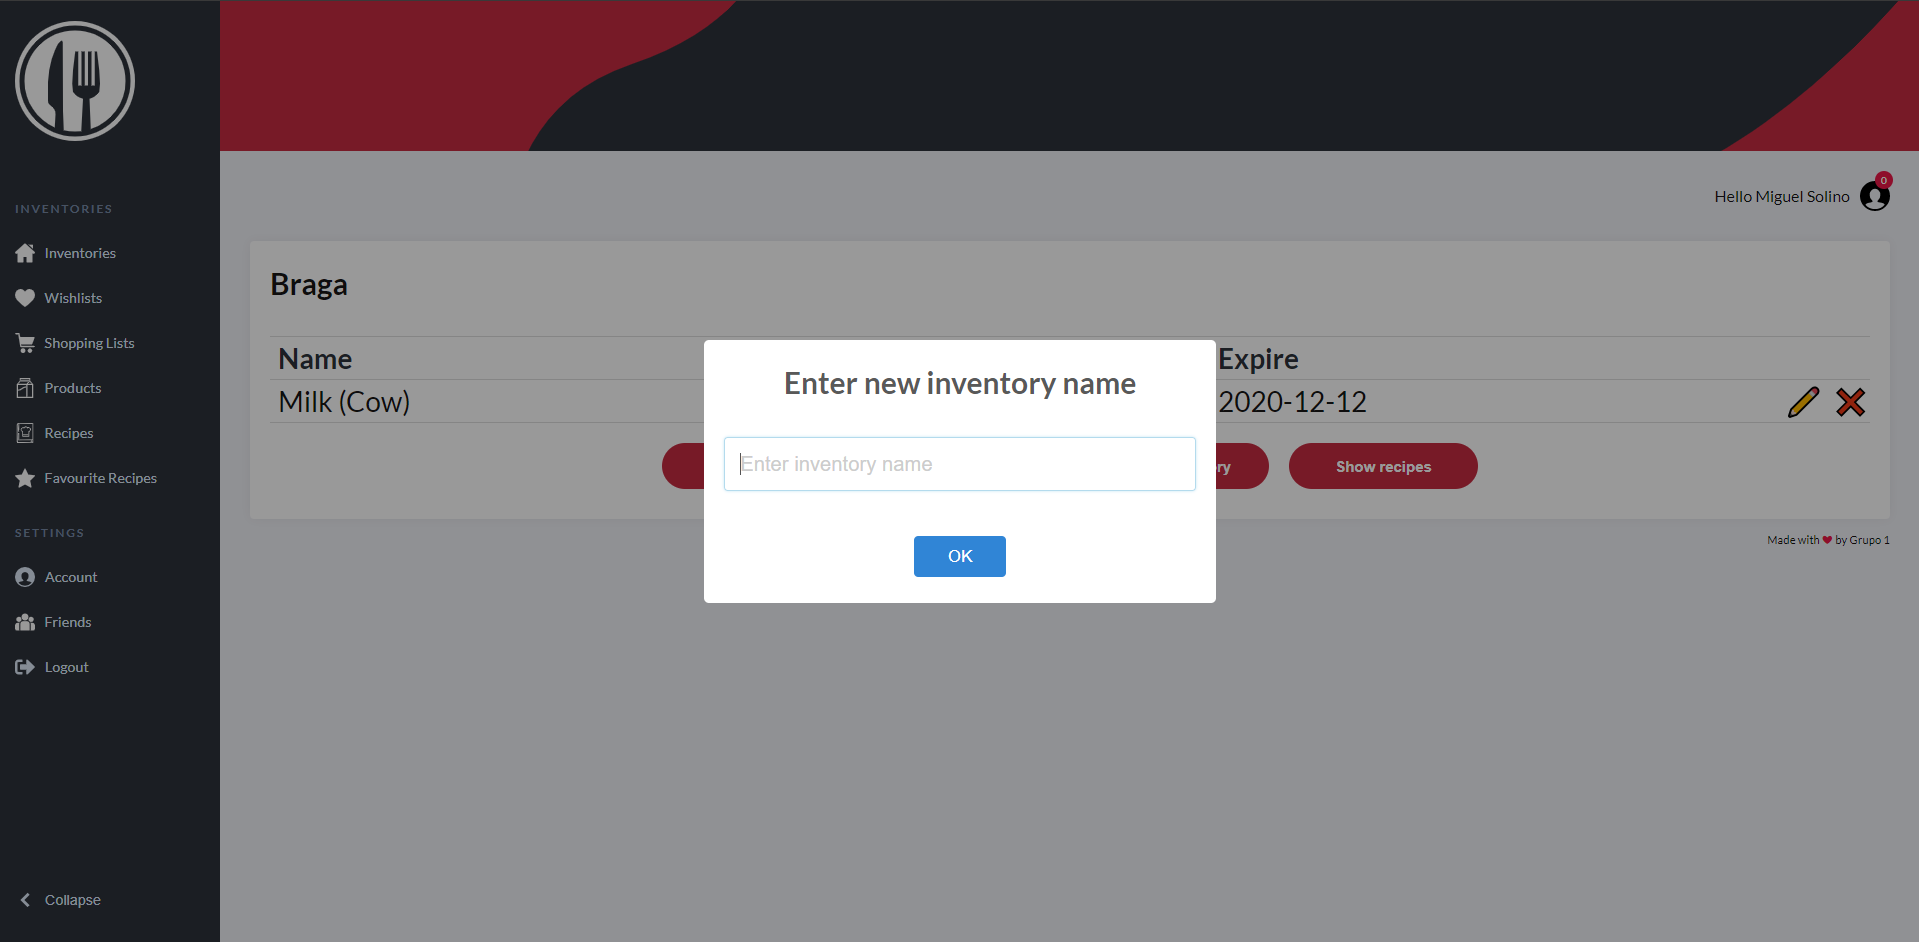
\includegraphics[width=\textwidth]{images/produto_final/alterar_nome_iventario.png}
    \end{figure}

    \begin{figure}[H]
        \centering
            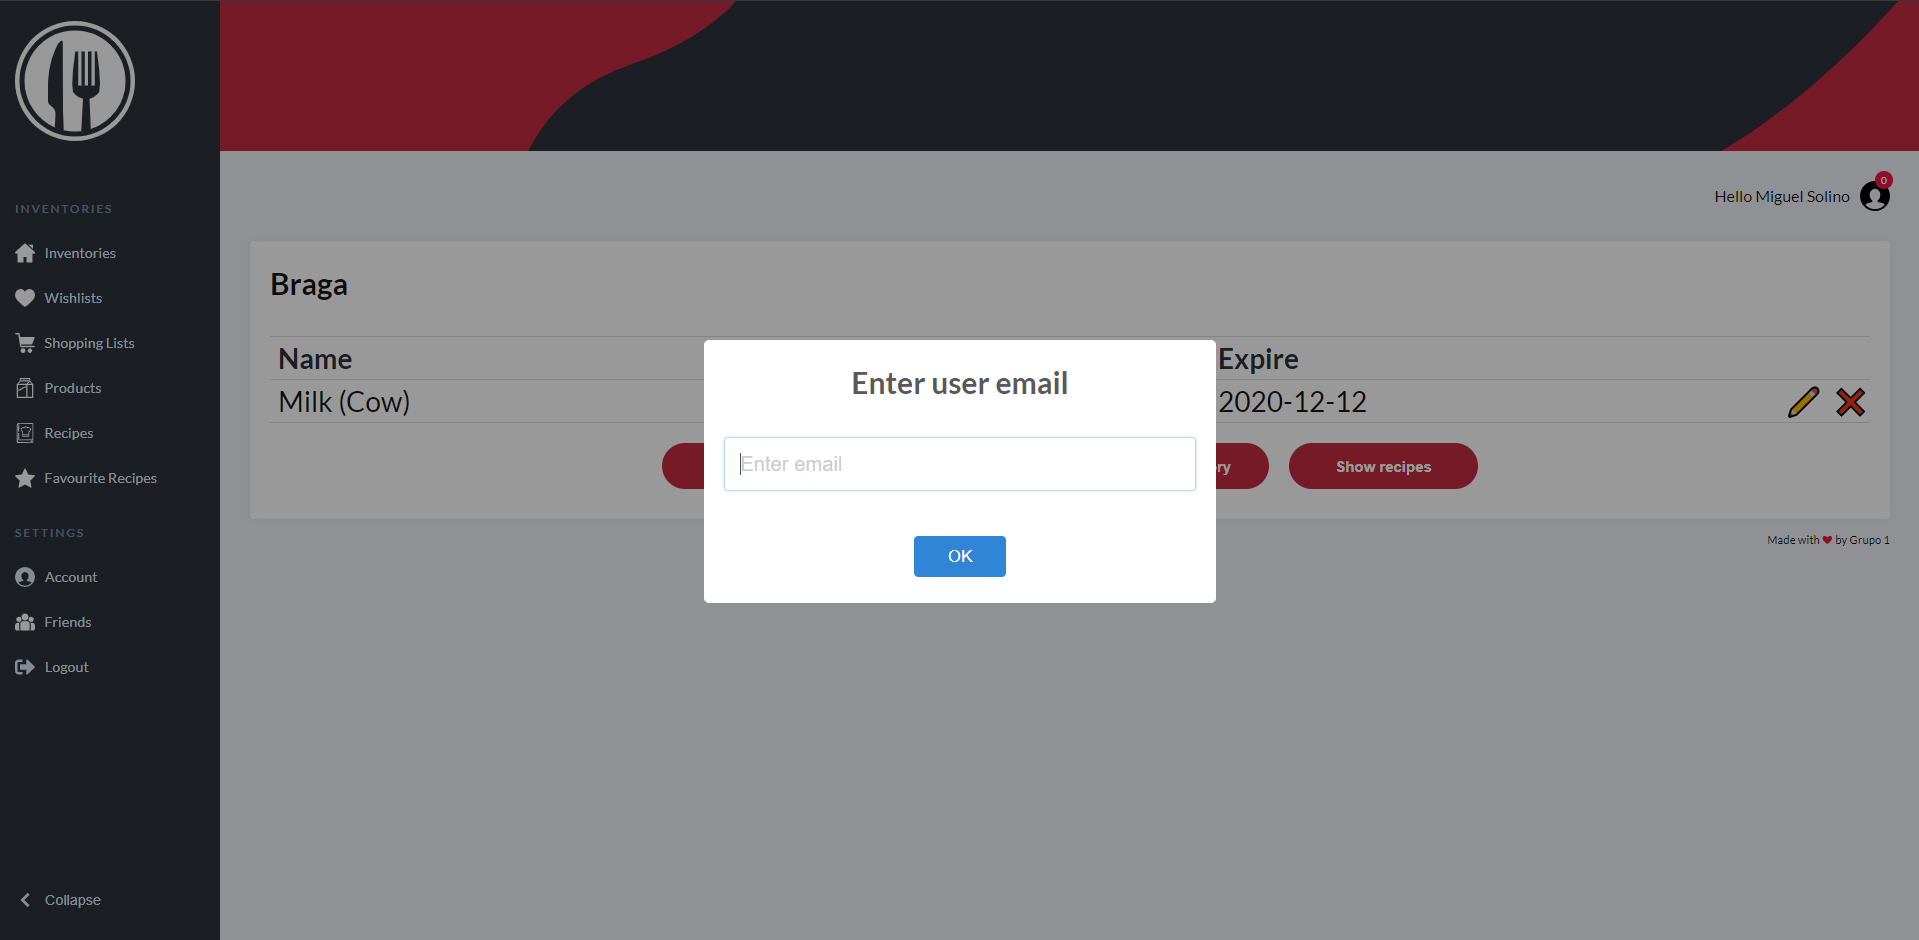
\includegraphics[width=\textwidth]{images/produto_final/partilhar_com_outro_utilizador.png}
    \end{figure}

    \begin{figure}[H]
        \centering
            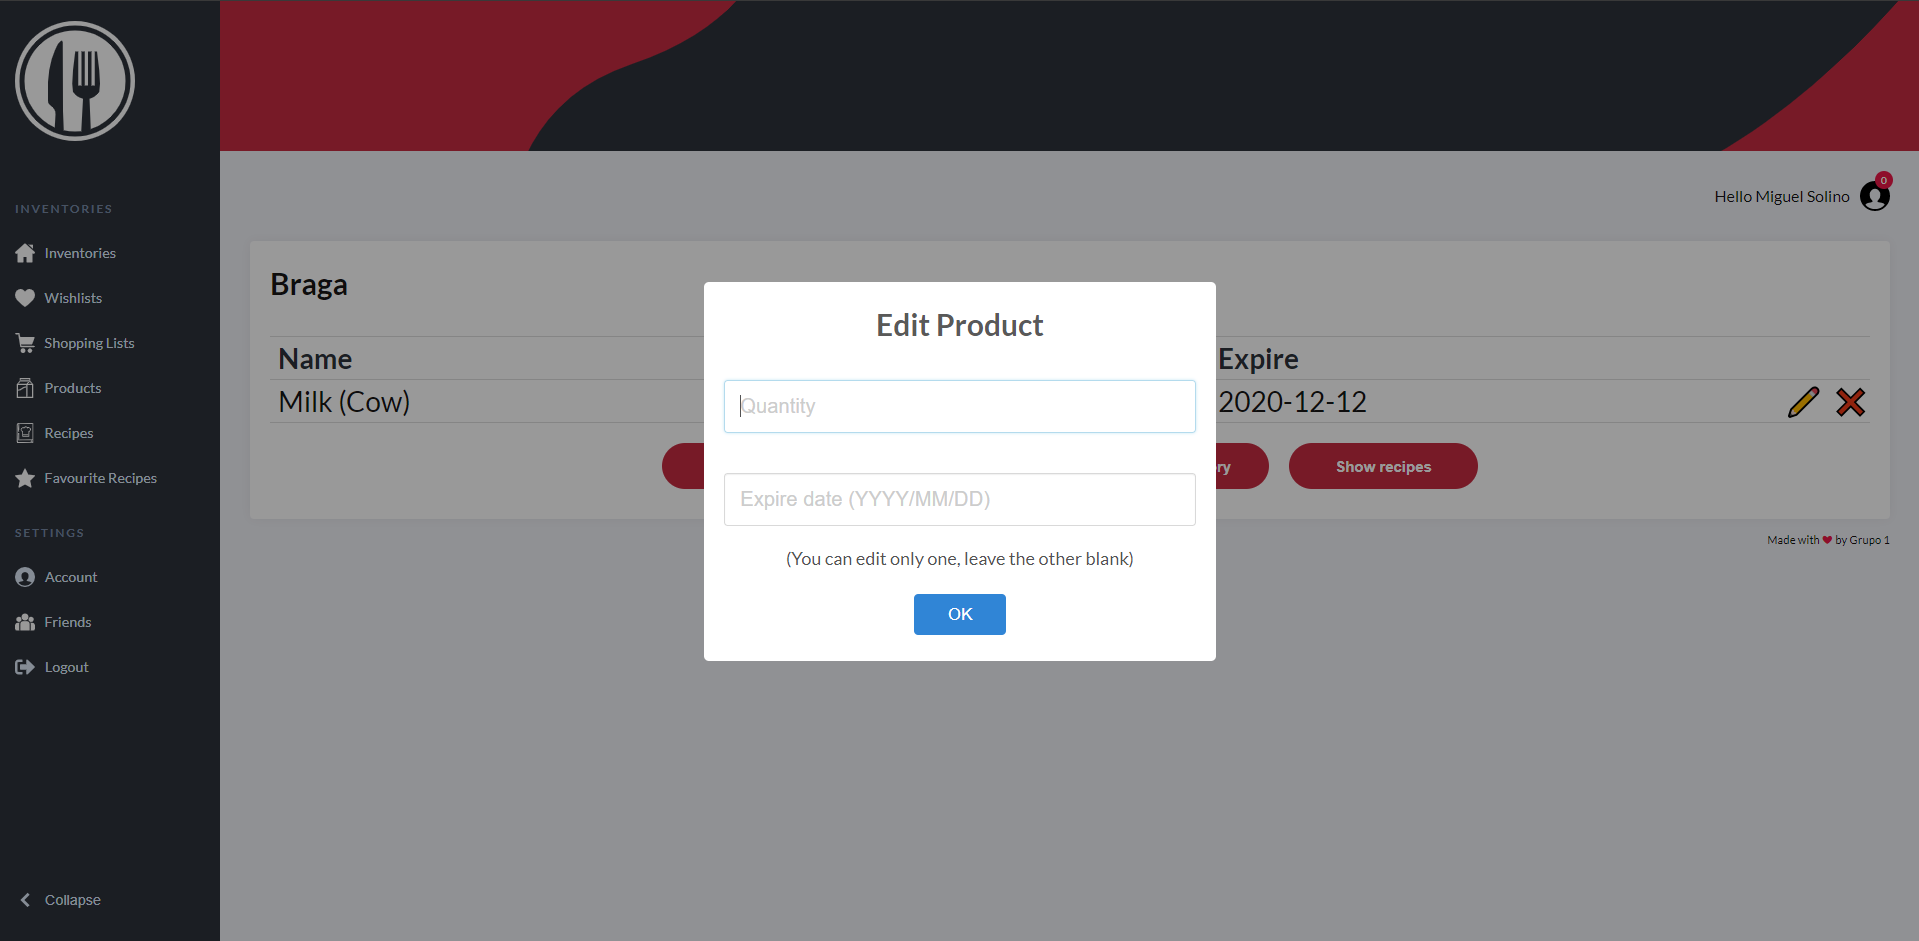
\includegraphics[width=\textwidth]{images/produto_final/editar_produto.png}
    \end{figure}

    \begin{figure}[H]
        \centering
            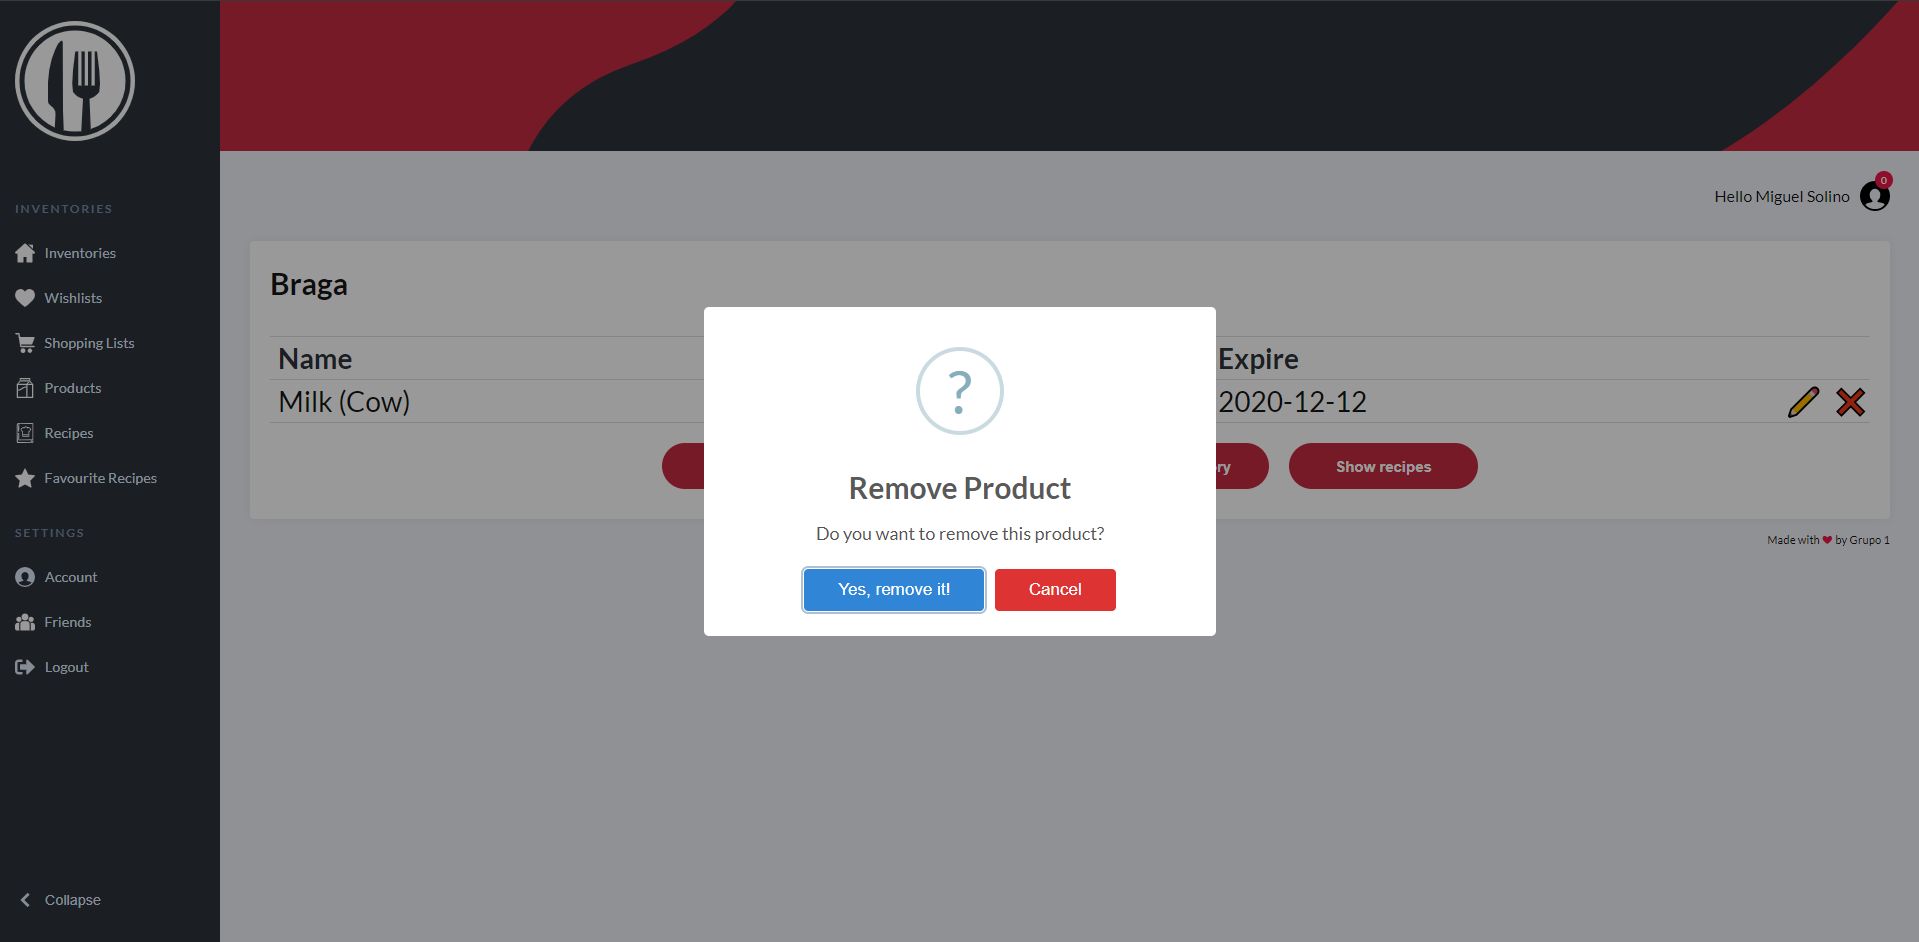
\includegraphics[width=\textwidth]{images/produto_final/eliminar_produto.png}
    \end{figure}

    \begin{figure}[H]
        \centering
            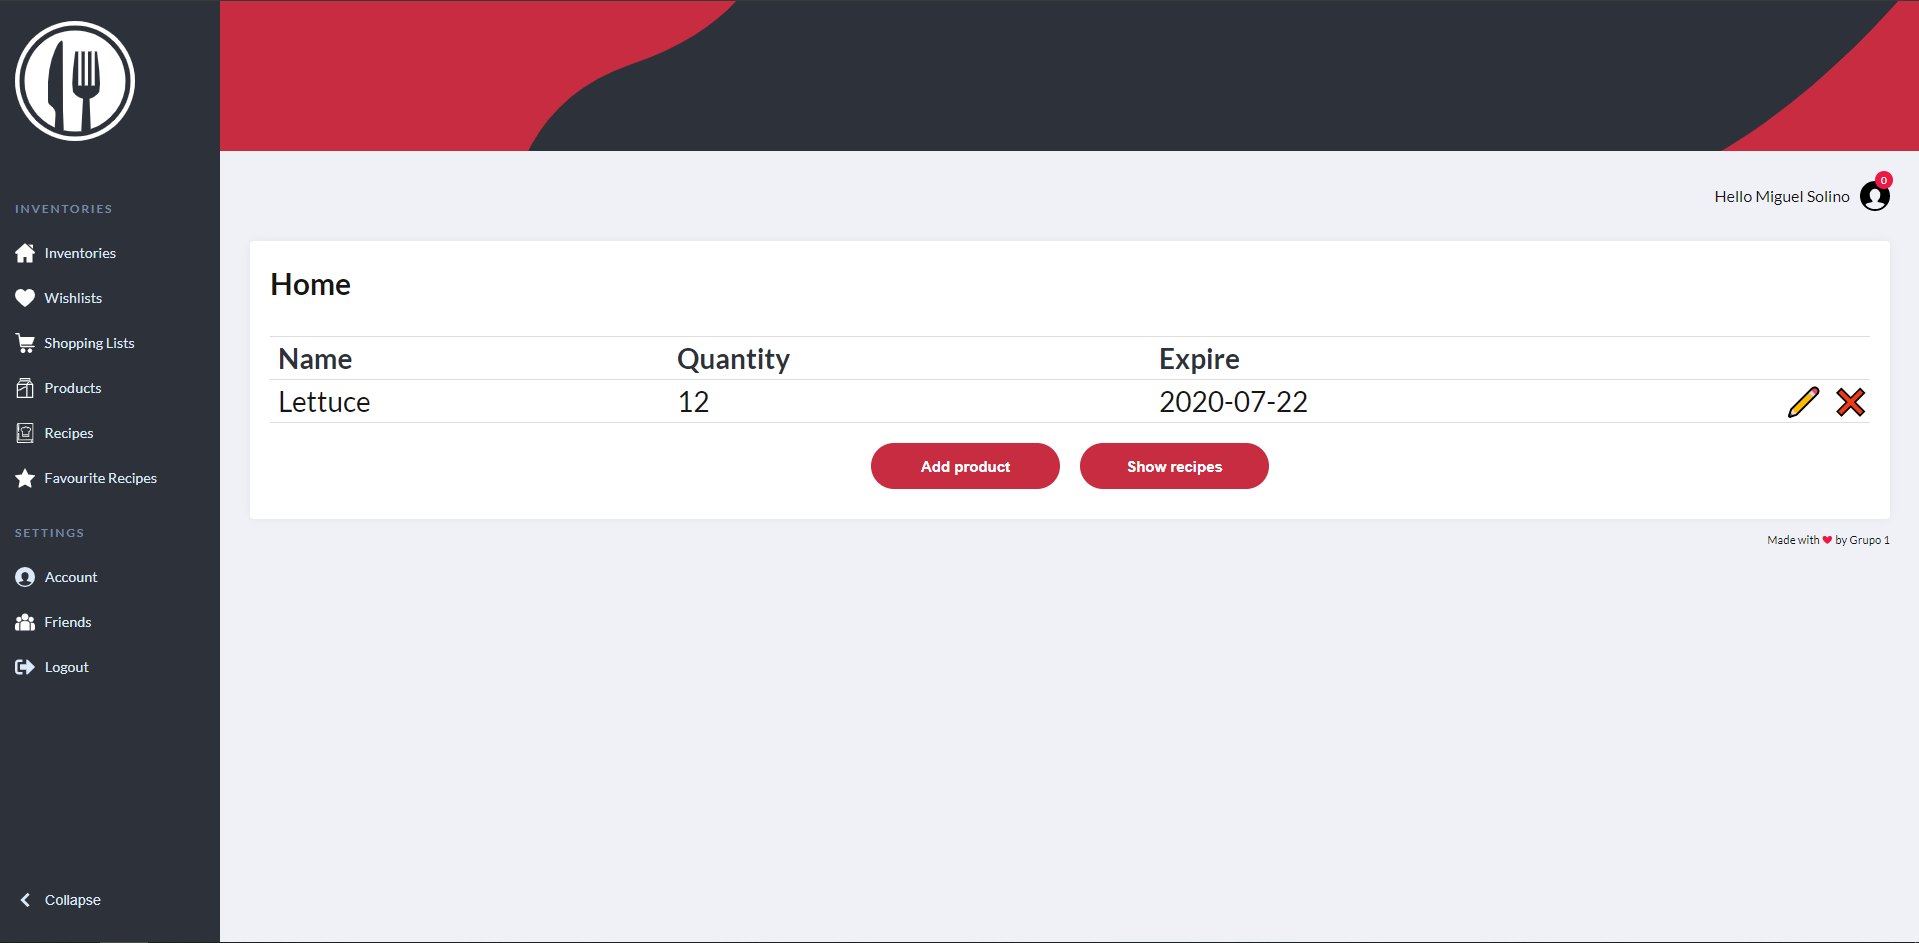
\includegraphics[width=\textwidth]{images/produto_final/pagina_iventario_partilhado.png}
    \end{figure}

    \begin{figure}[H]
        \centering
            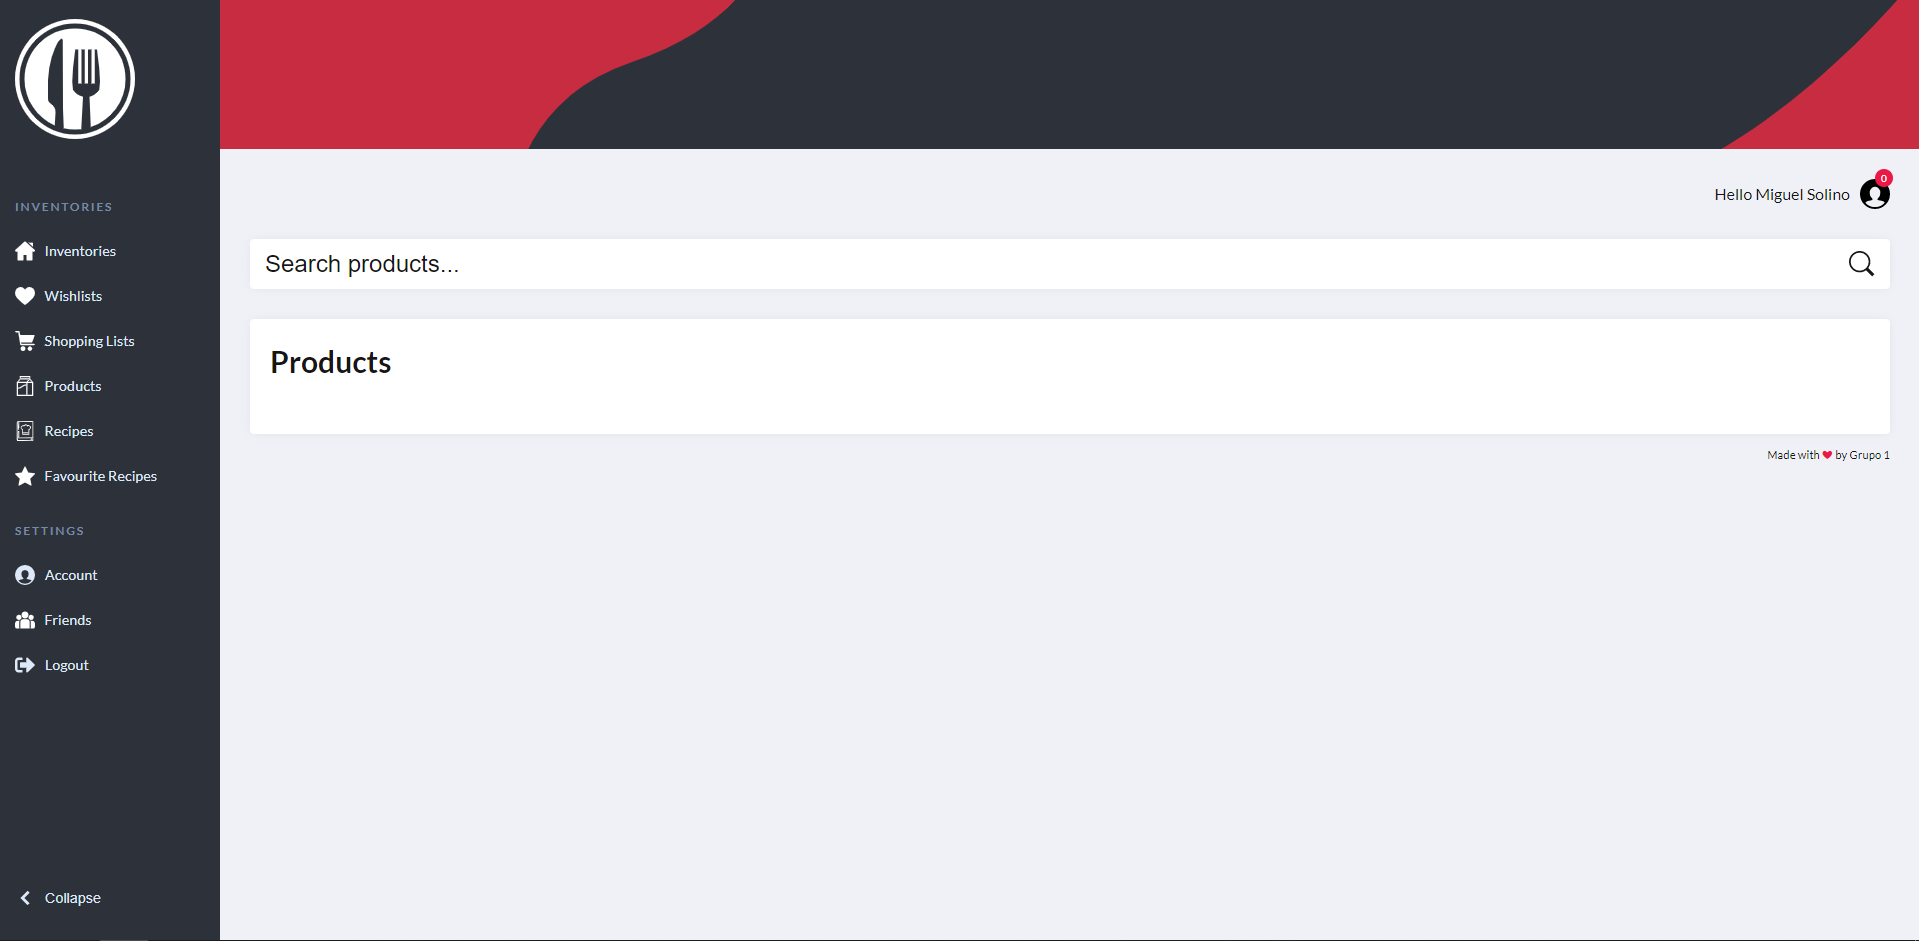
\includegraphics[width=\textwidth]{images/produto_final/procura_de_produtos.png}
    \end{figure}

    \begin{figure}[H]
        \centering
            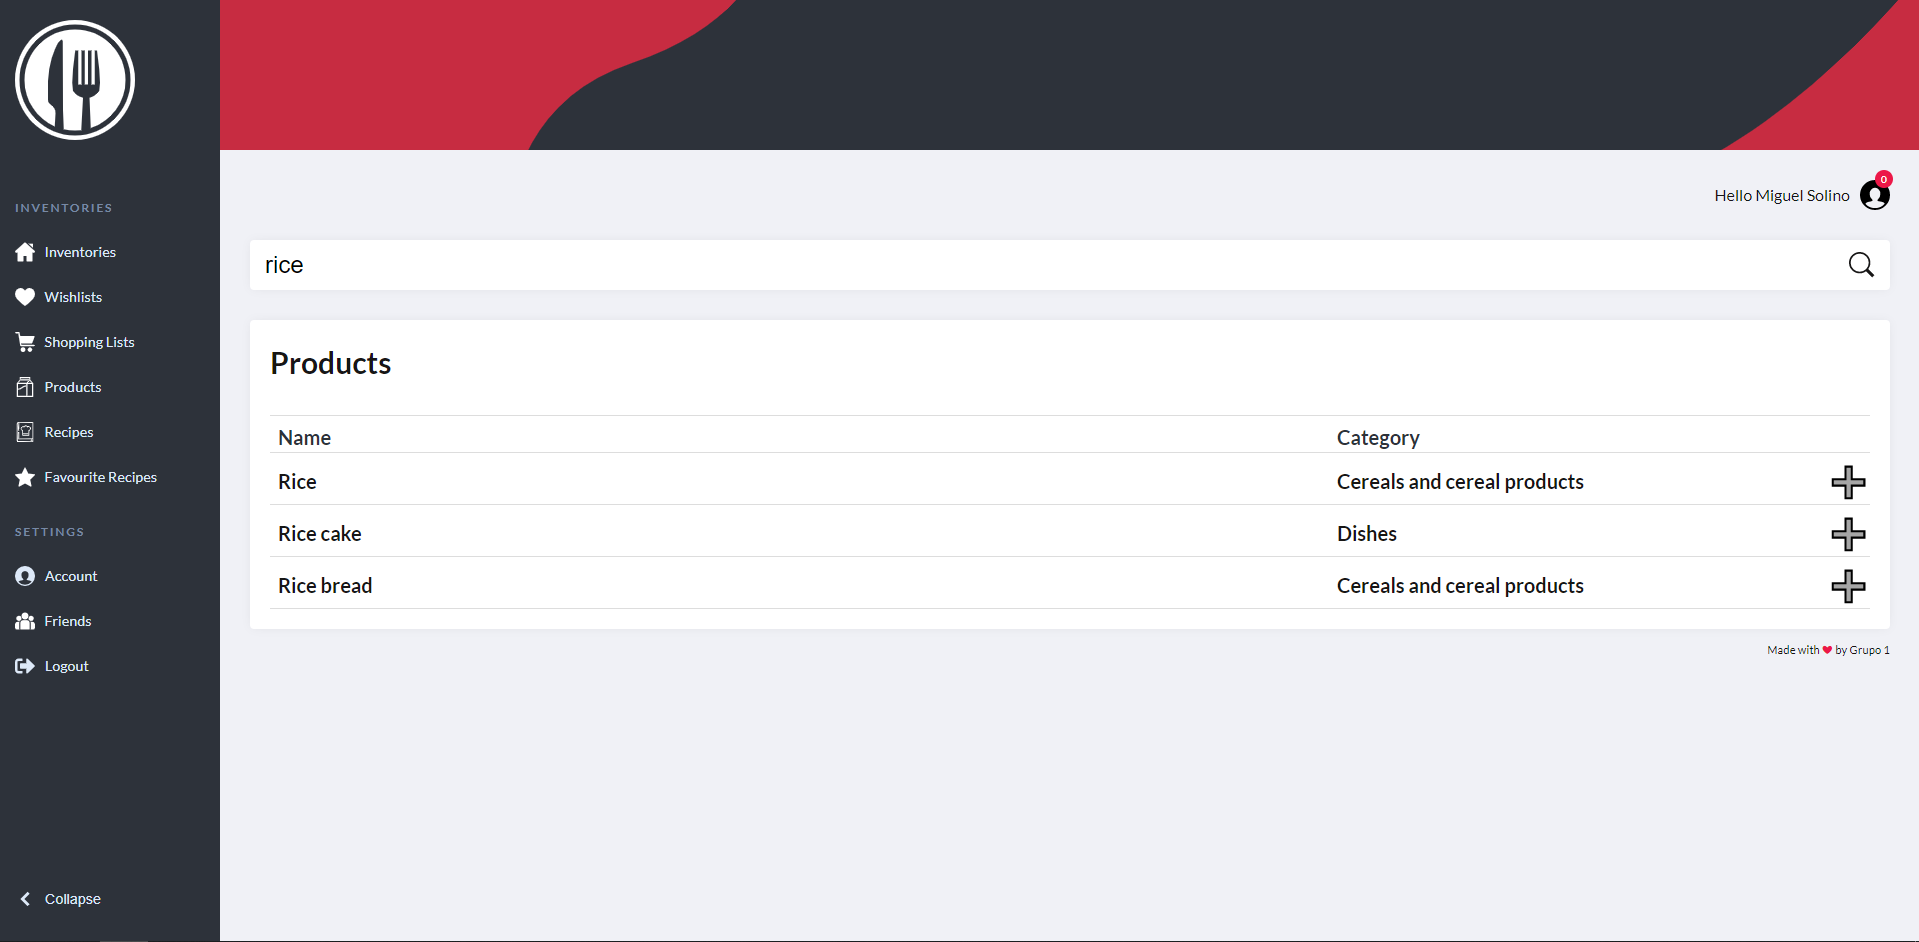
\includegraphics[width=\textwidth]{images/produto_final/procura_de_produtos_efetuada.png}
    \end{figure}

    \begin{figure}[H]
        \centering
            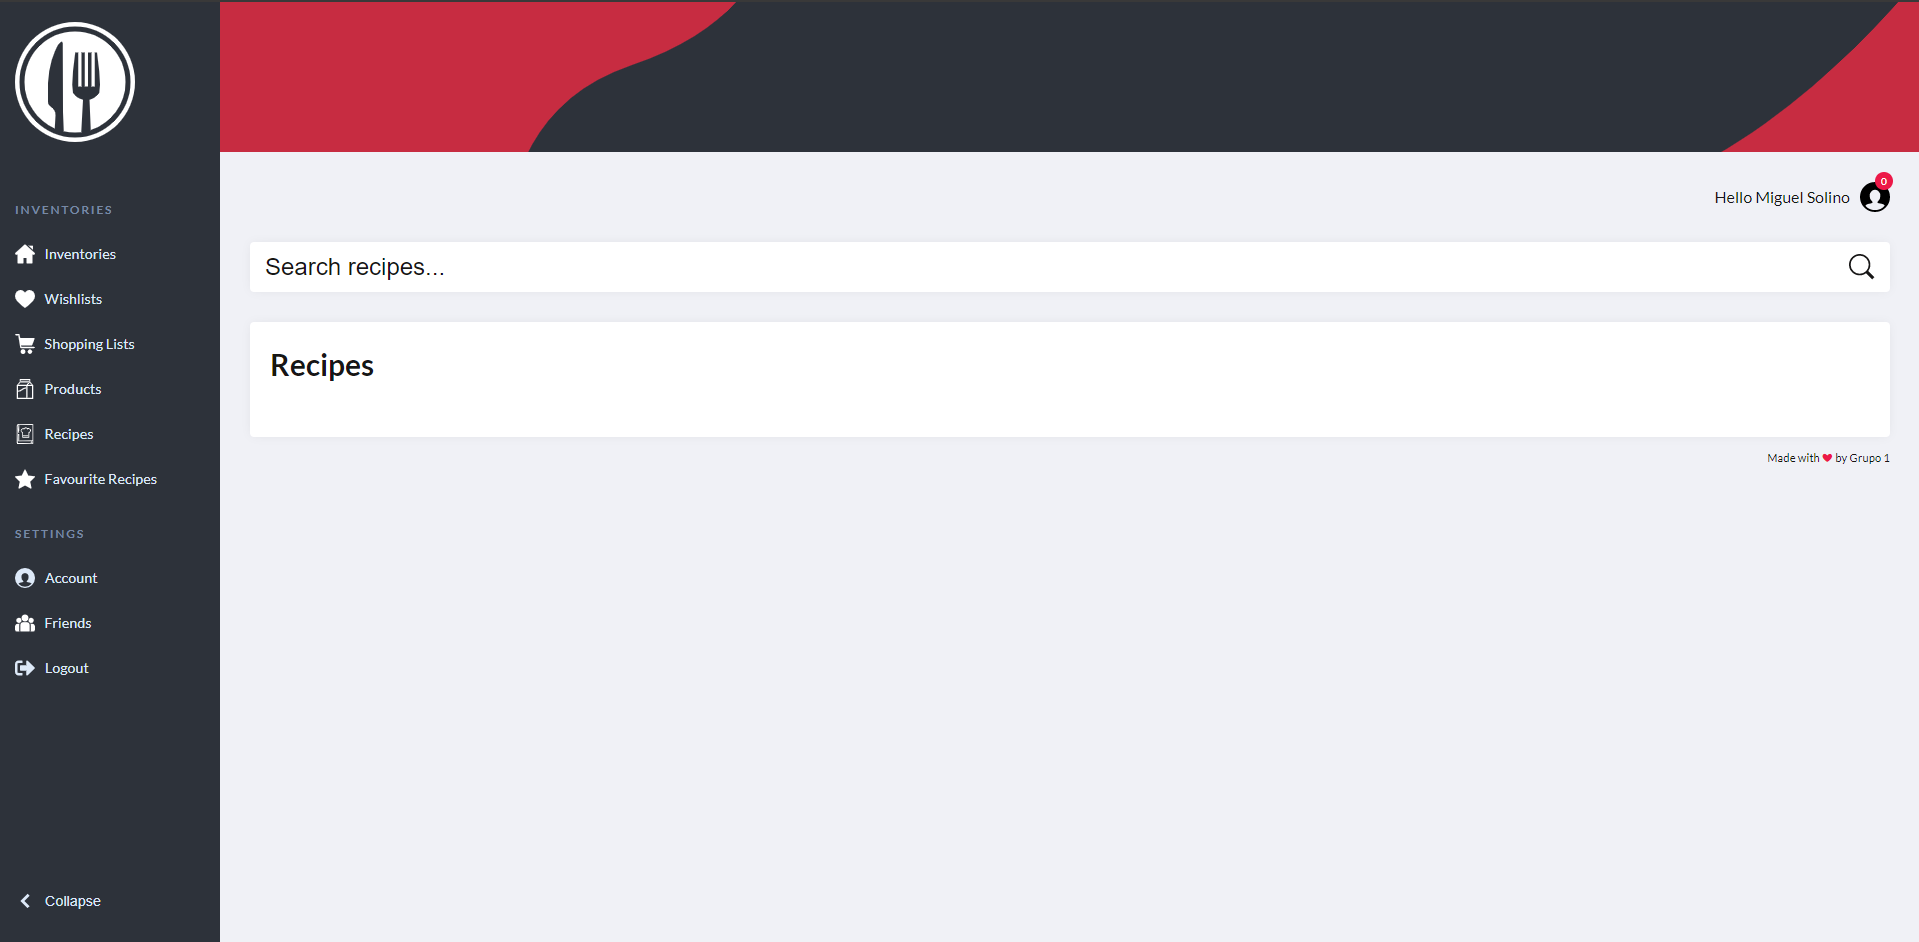
\includegraphics[width=\textwidth]{images/produto_final/procura_de_receitas.png}
    \end{figure}

    \begin{figure}[H]
        \centering
            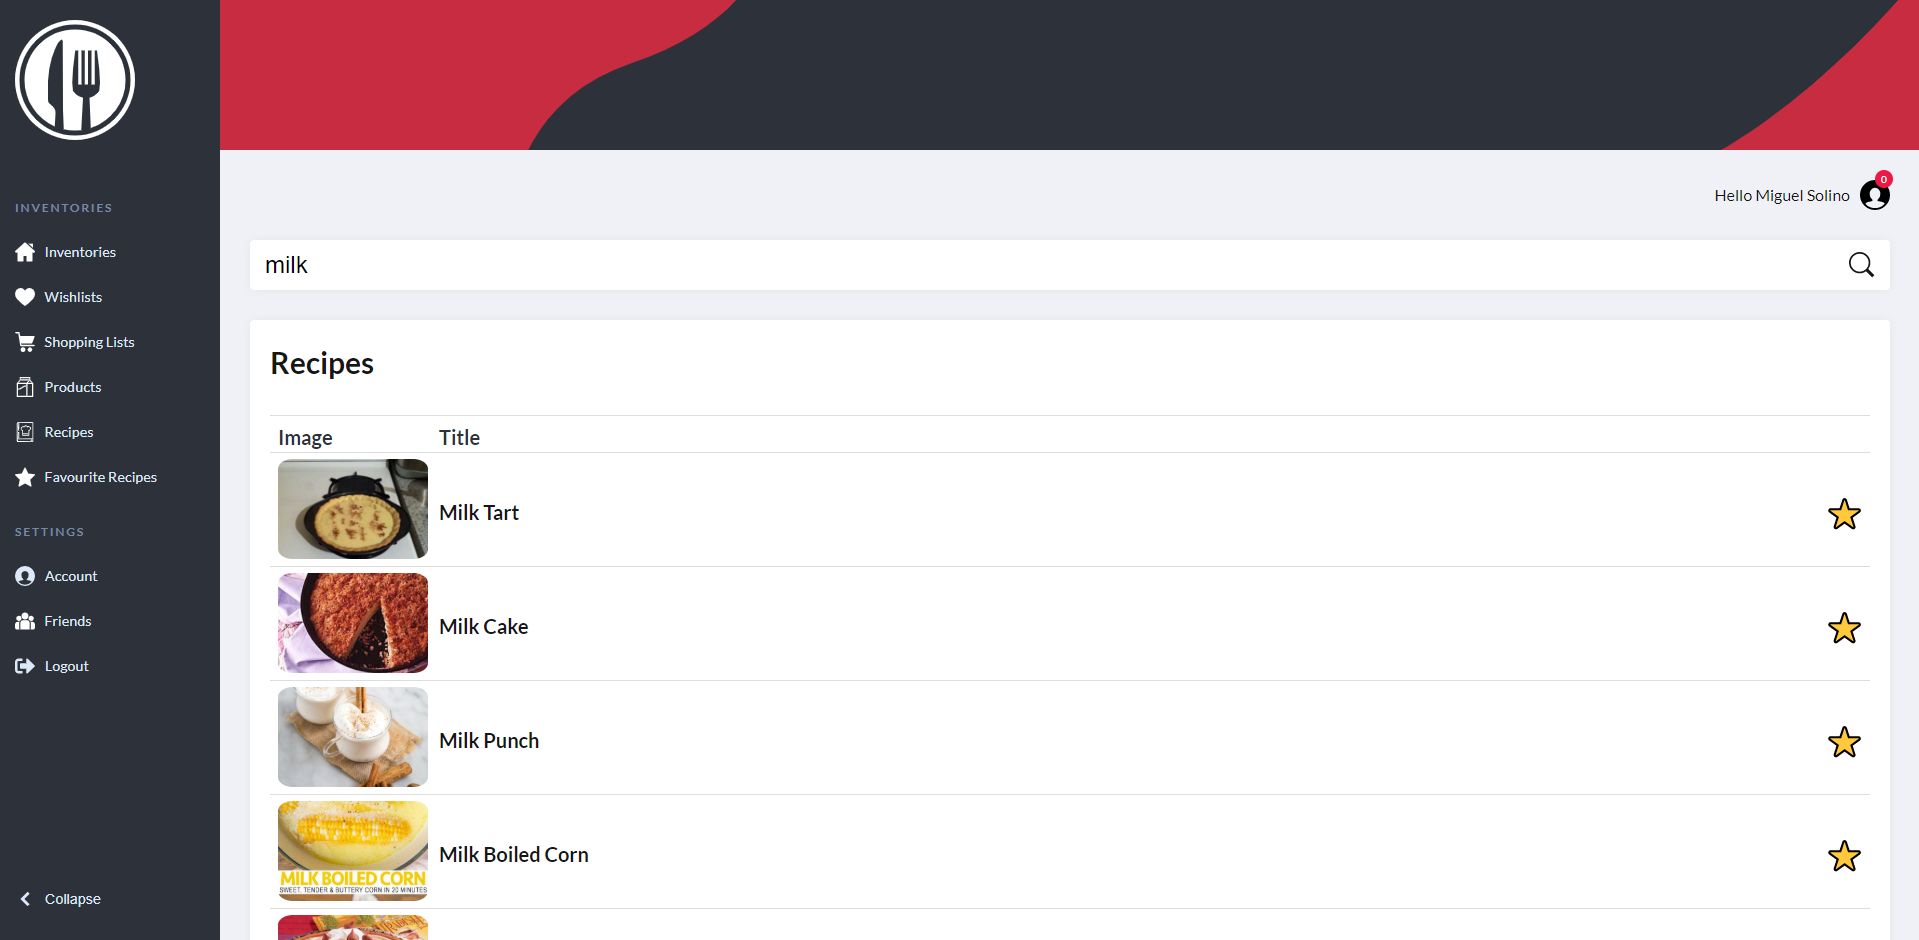
\includegraphics[width=\textwidth]{images/produto_final/procura_de_receitas_efetuadas.png}
    \end{figure}

    \begin{figure}[H]
        \centering
            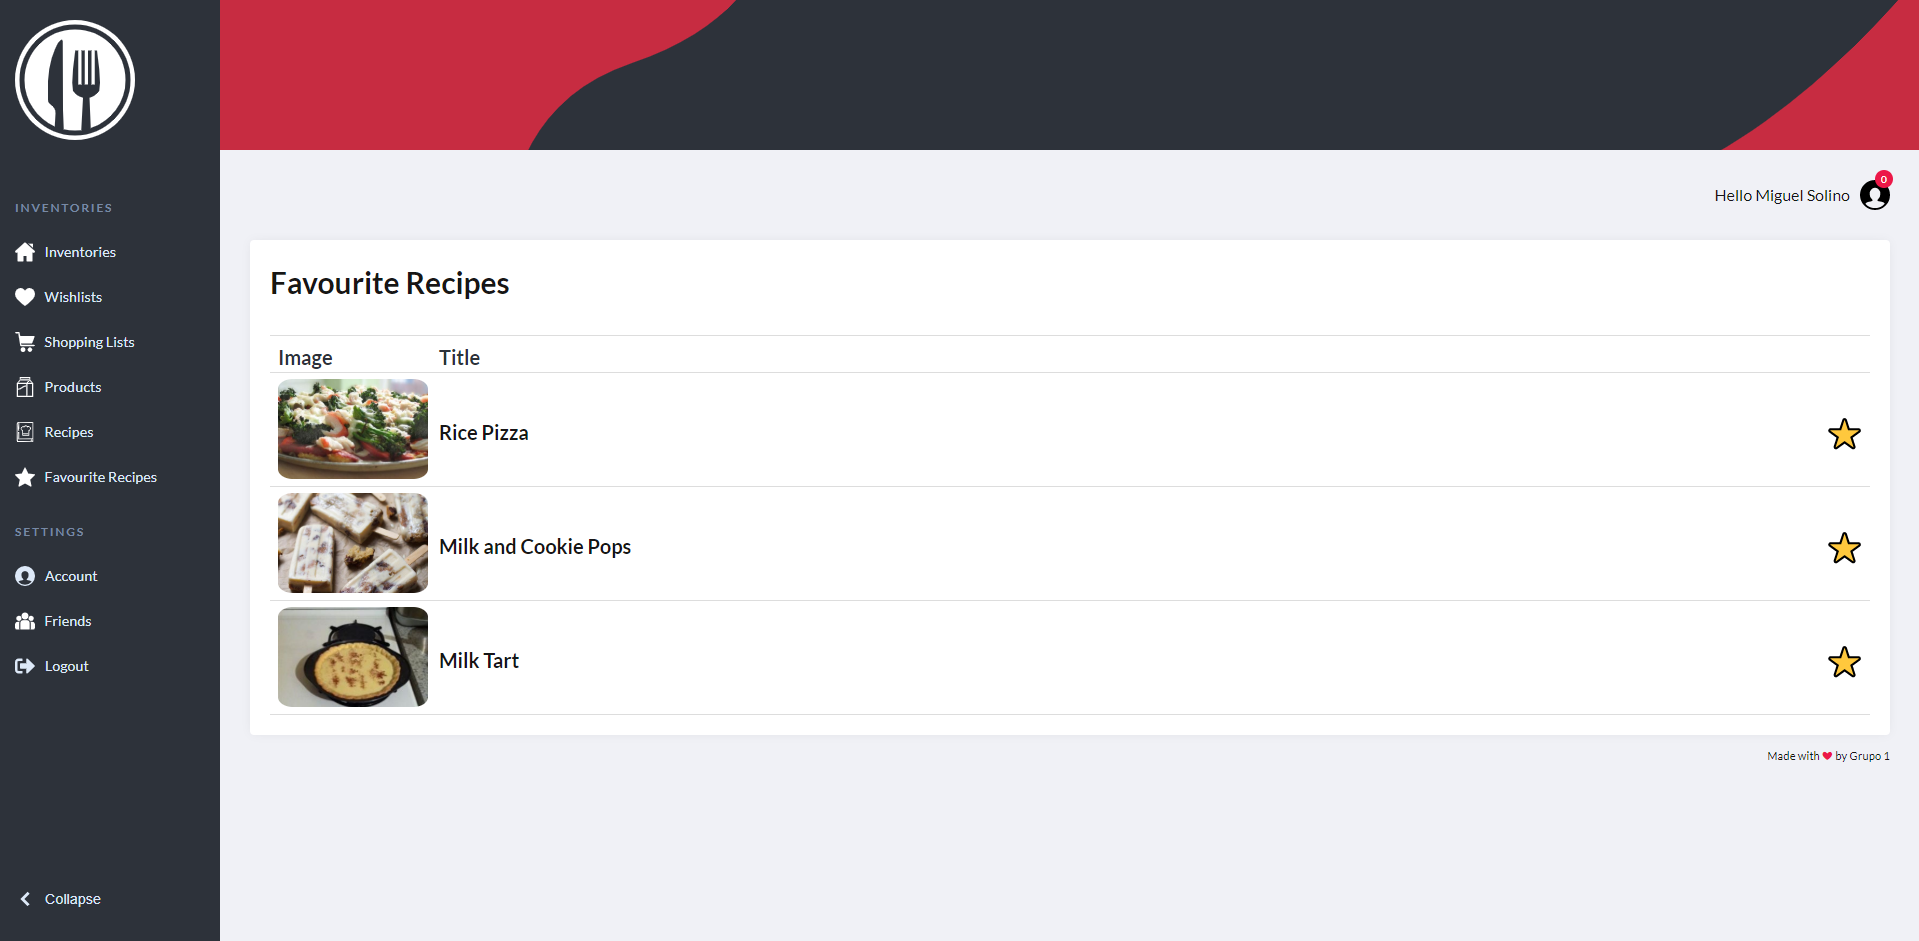
\includegraphics[width=\textwidth]{images/produto_final/receitas_favoritas.png}
    \end{figure}

    \begin{figure}[H]
        \centering
            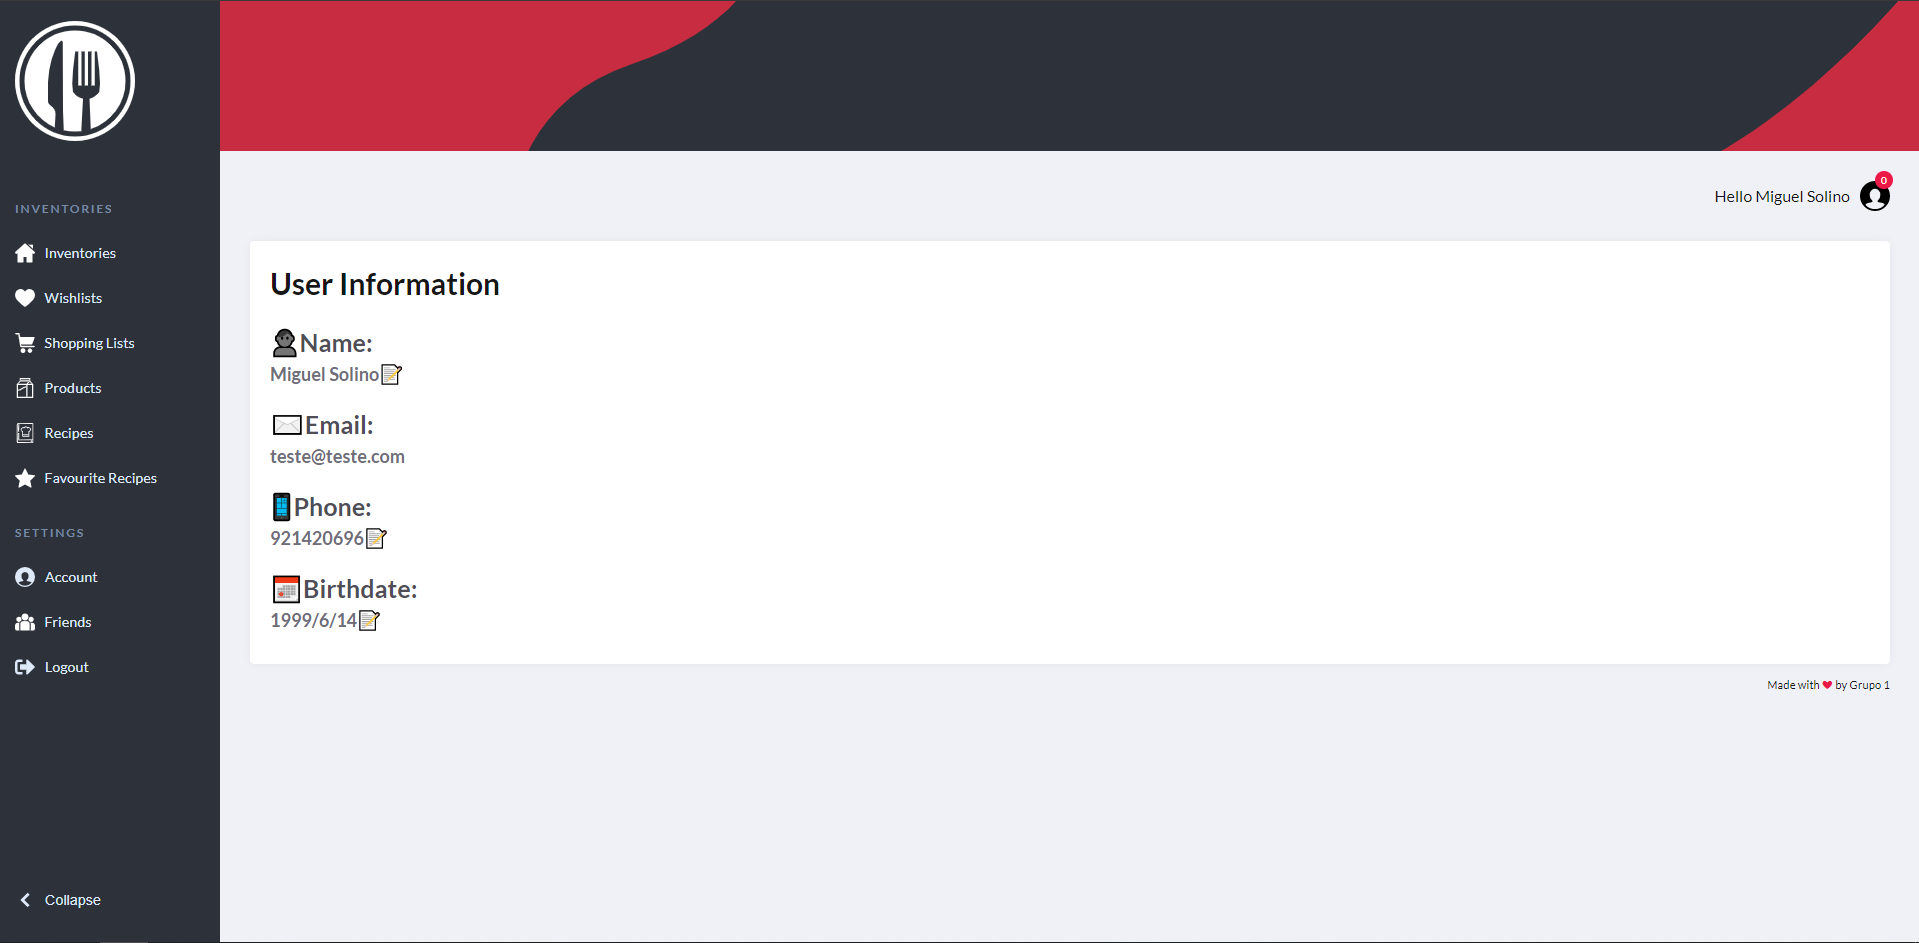
\includegraphics[width=\textwidth]{images/produto_final/pagina_de_perfil.png}
    \end{figure}

    \begin{figure}[H]
        \centering
            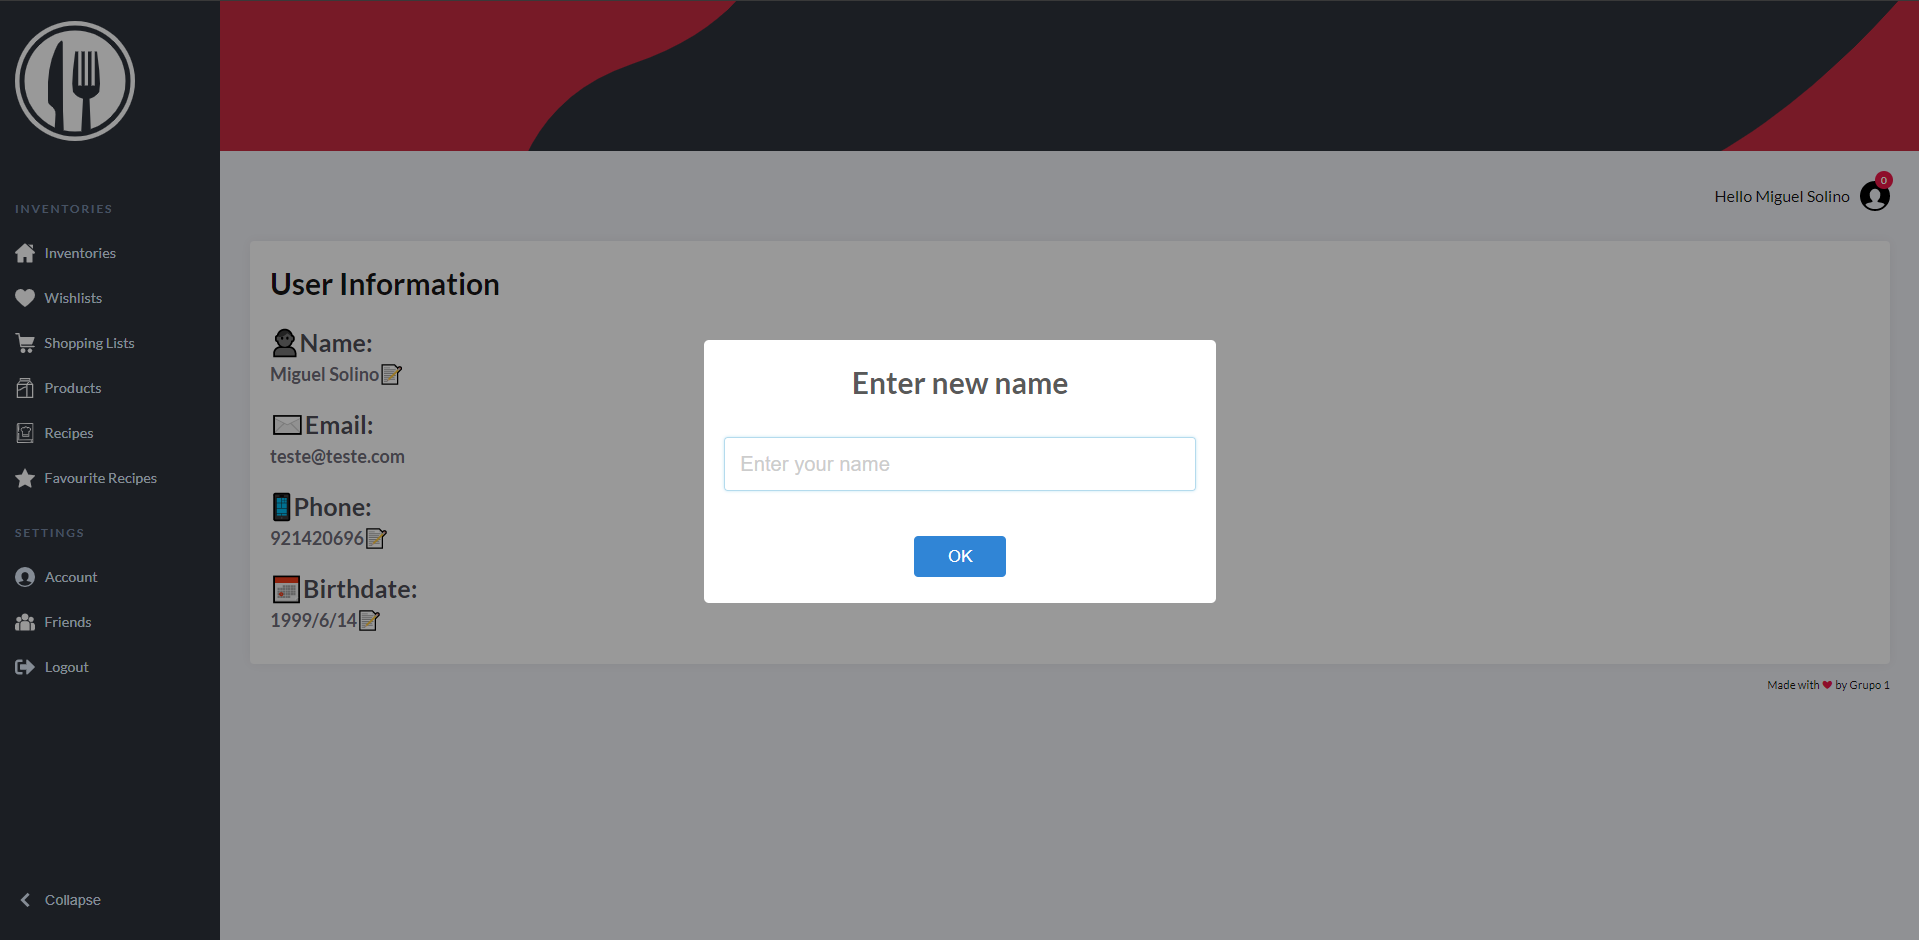
\includegraphics[width=\textwidth]{images/produto_final/alterar_nome_perfil.png}
    \end{figure}

    \begin{figure}[H]
        \centering
            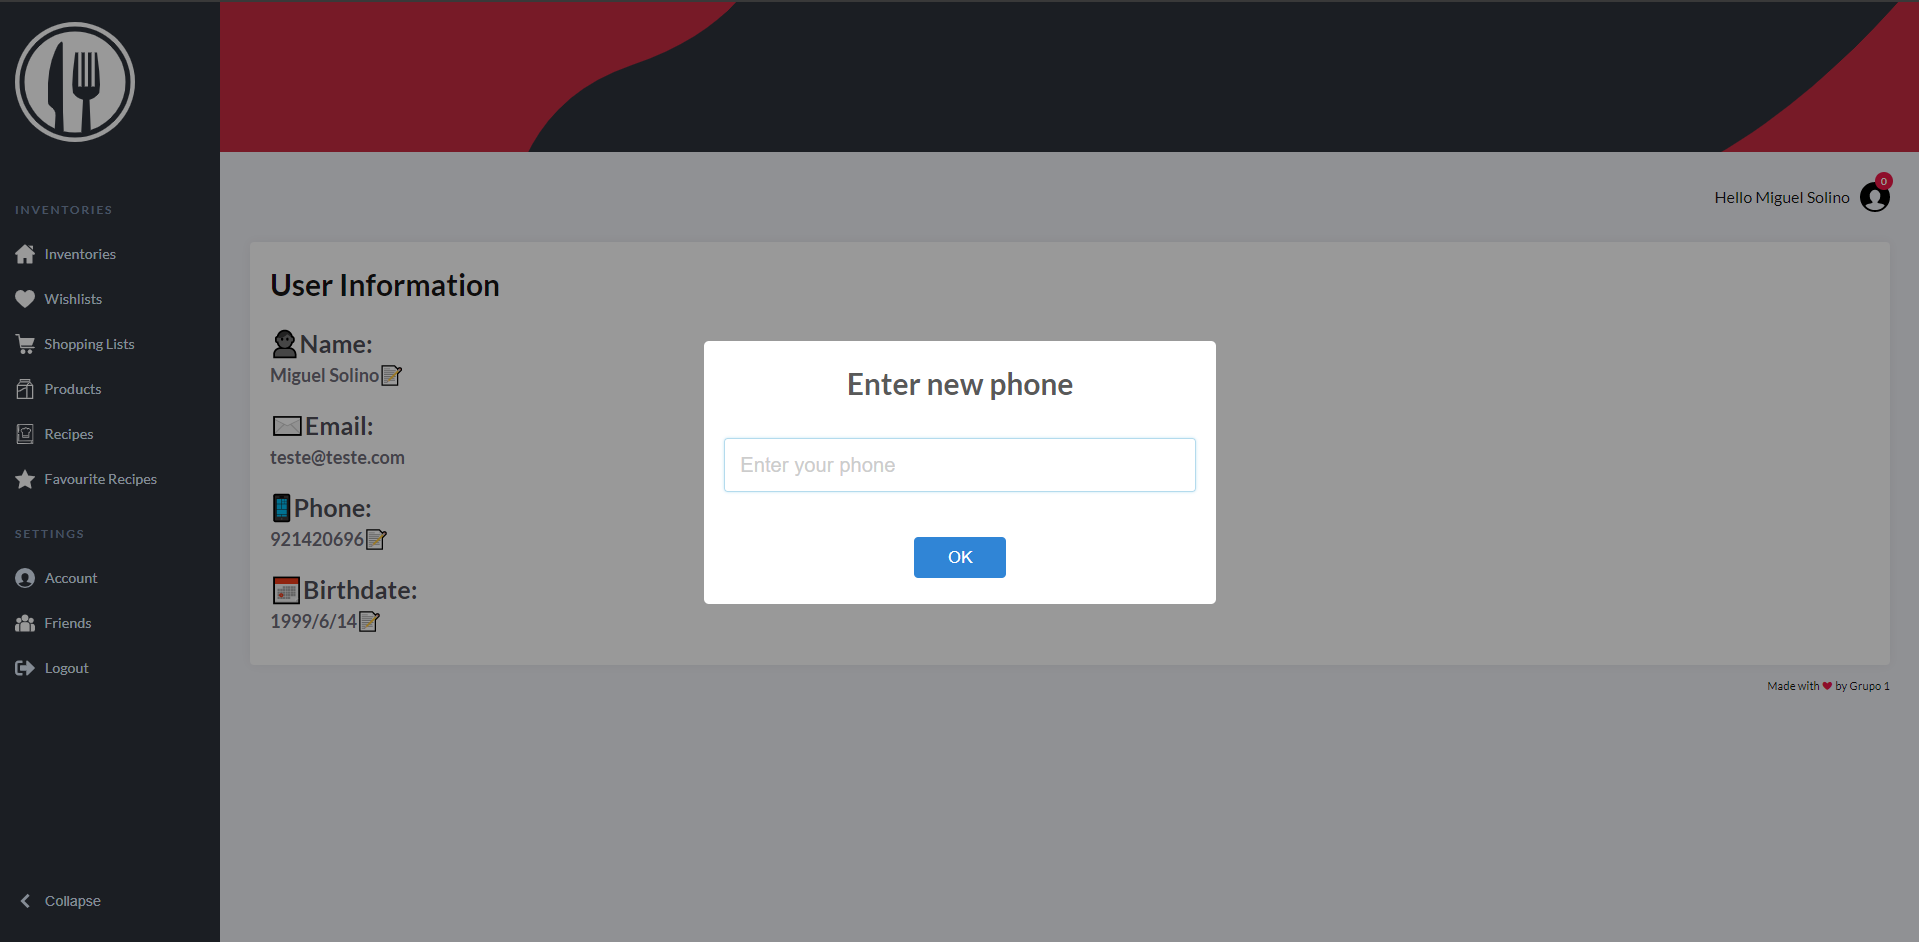
\includegraphics[width=\textwidth]{images/produto_final/alterar_numero_perfil.png}
    \end{figure}

    \begin{figure}[H]
        \centering
            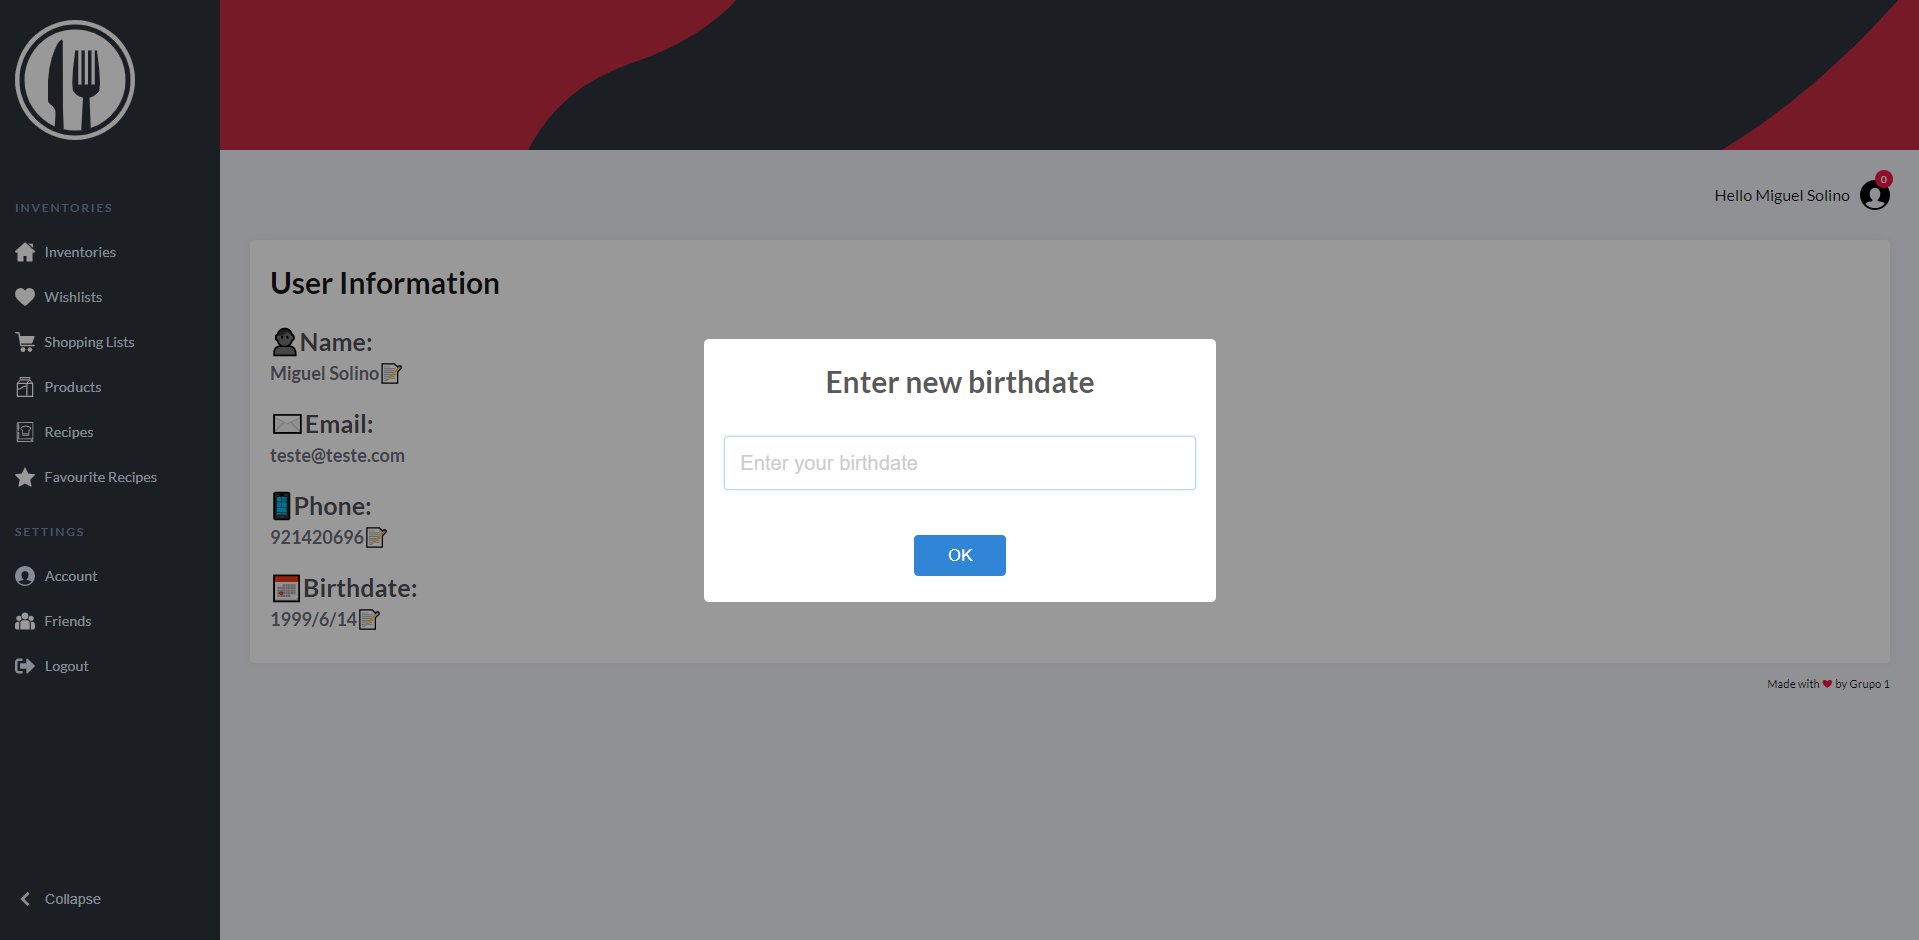
\includegraphics[width=\textwidth]{images/produto_final/alterar_nascimento_iventario.png}
    \end{figure}

    \begin{figure}[H]
        \centering
            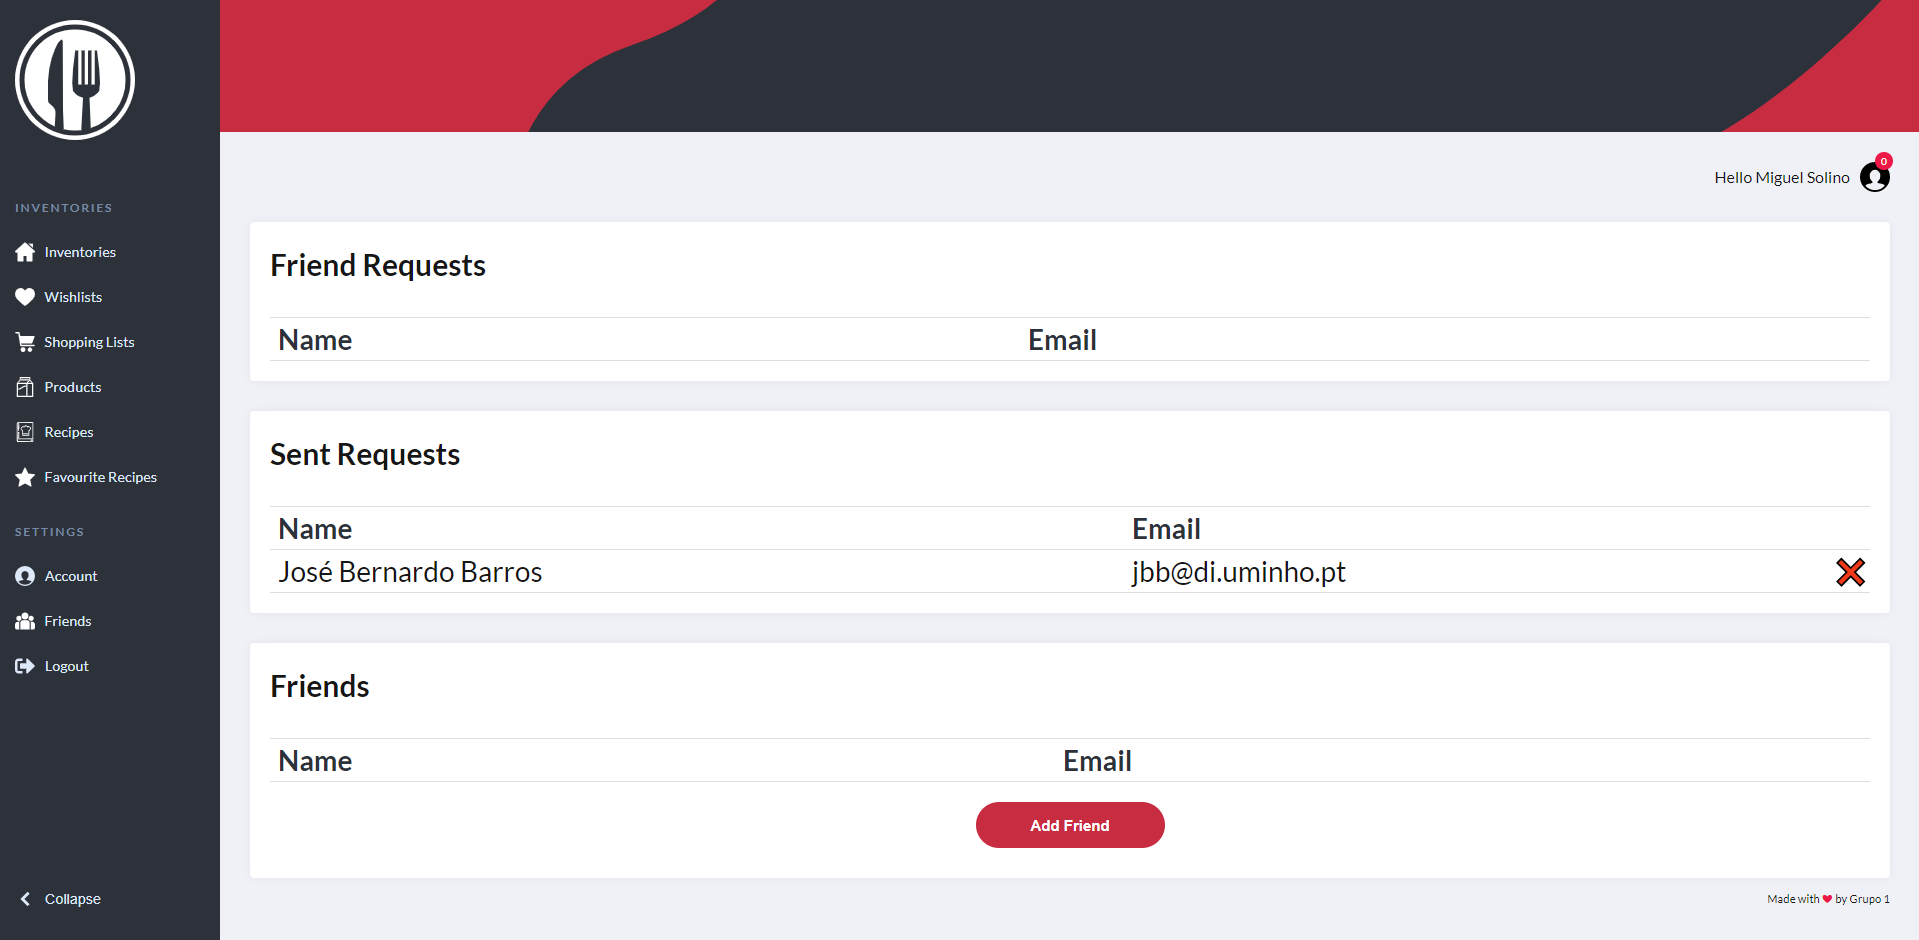
\includegraphics[width=\textwidth]{images/produto_final/pedido_amigos_enviado.png}
    \end{figure}

    \begin{figure}[H]
        \centering
            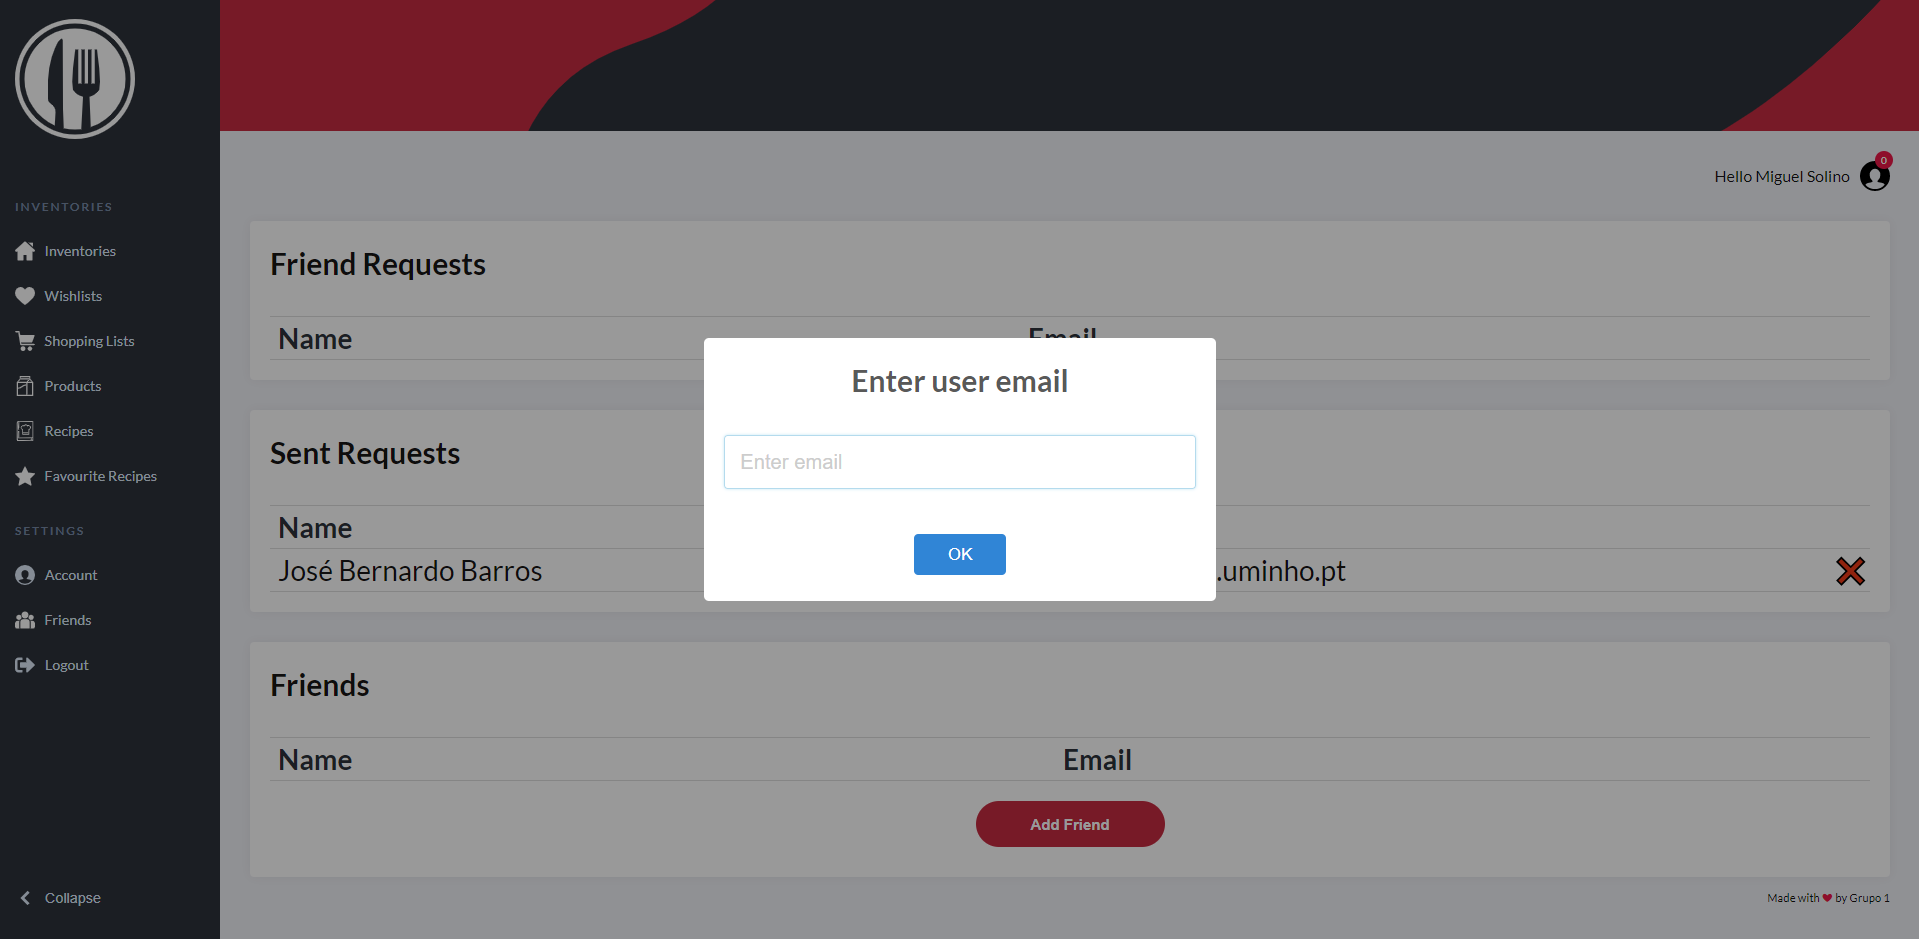
\includegraphics[width=\textwidth]{images/produto_final/adicionar_amigo.png}
    \end{figure}

    \begin{figure}[H]
        \centering
            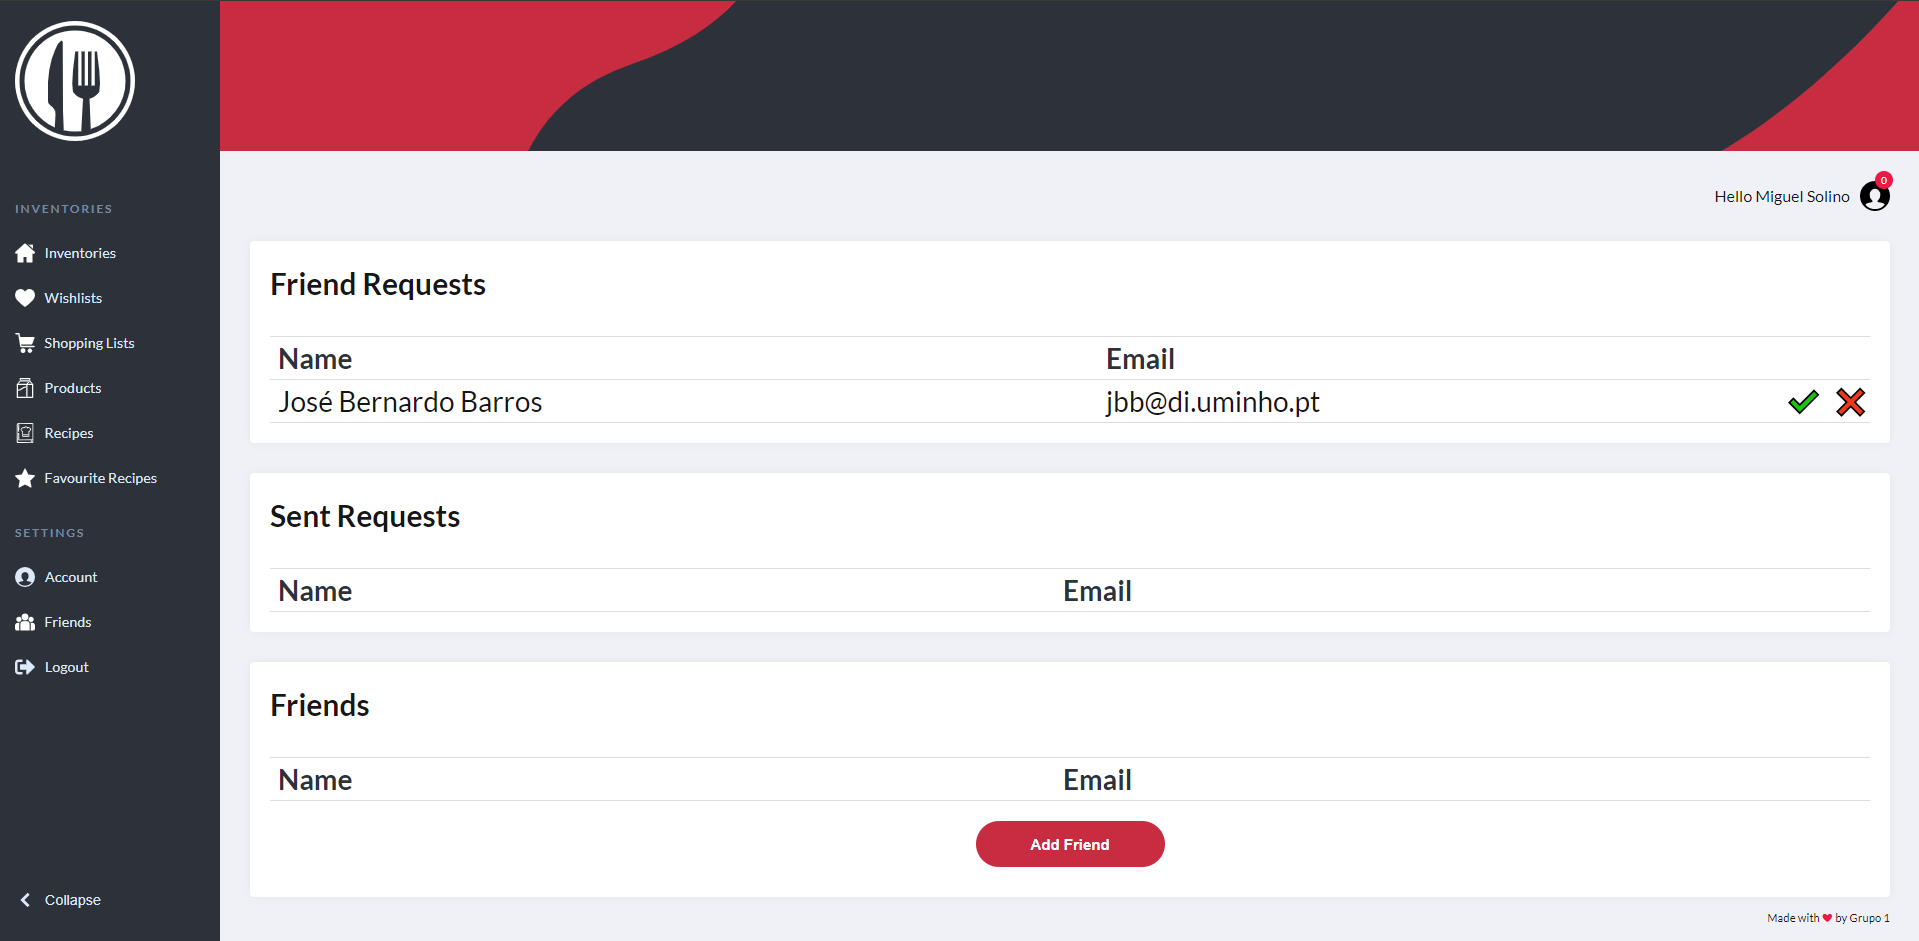
\includegraphics[width=\textwidth]{images/produto_final/pedido_recebido.png}
    \end{figure}

    \begin{figure}[H]
        \centering
            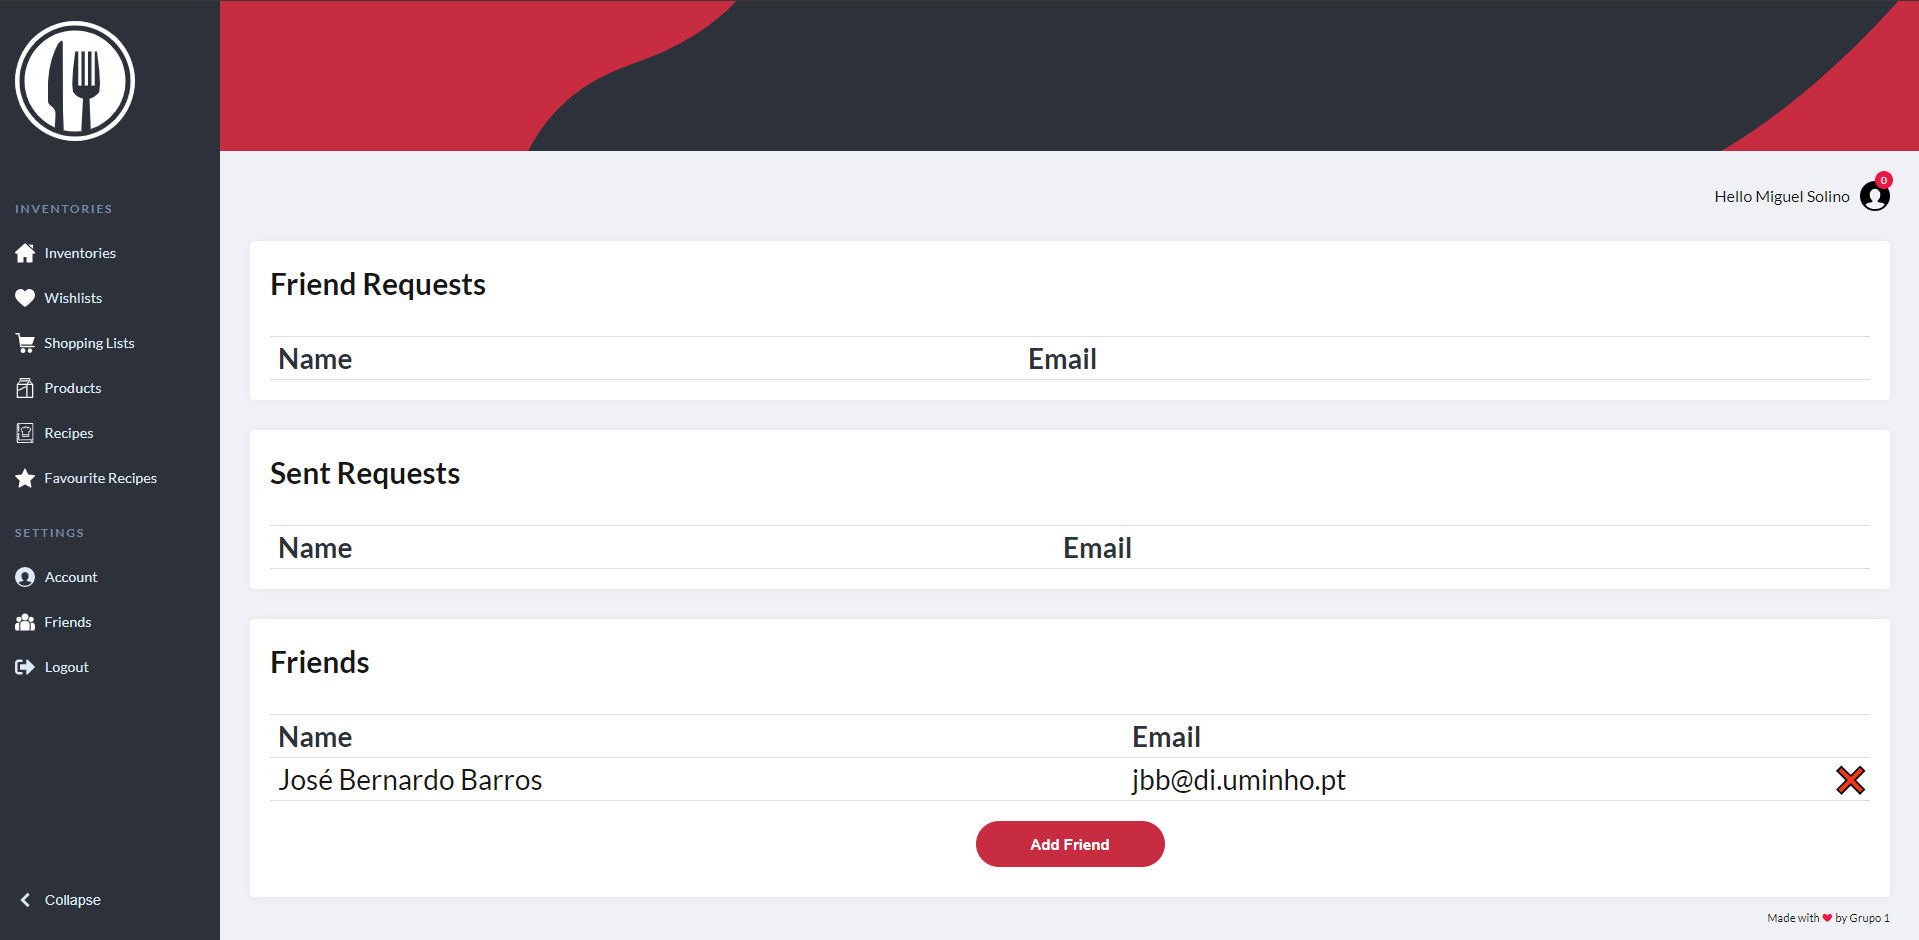
\includegraphics[width=\textwidth]{images/produto_final/amigo_adicionado.png}
    \end{figure}

    \begin{figure}[H]
        \centering
            \includegraphics[width=\textwidth]{images/produto_final/exemplo_erro.png}
    \end{figure}

    \begin{figure}[H]
        \centering
            \includegraphics[width=\textwidth]{images/produto_final/exemplo_sucesso.png}
    \end{figure}

\chapter{Conclusões}

\chapter{Referências}

\chapter{Lista de Siglas e Acrónimos}

\end{document}
